%%
%% This is file `sample-sigconf.tex',
%% generated with the docstrip utility.
%%
%% The original source files were:
%%
%% samples.dtx  (with options: `sigconf')
%% 
%% IMPORTANT NOTICE:
%% 
%% For the copyright see the source file.
%% 
%% Any modified versions of this file must be renamed
%% with new filenames distinct from sample-sigconf.tex.
%% 
%% For distribution of the original source see the terms
%% for copying and modification in the file samples.dtx.
%% 
%% This generated file may be distributed as long as the
%% original source files, as listed above, are part of the
%% same distribution. (The sources need not necessarily be
%% in the same archive or directory.)
%%
%%
%% Commands for TeXCount
%TC:macro \cite [option:text,text]
%TC:macro \citep [option:text,text]
%TC:macro \citet [option:text,text]
%TC:envir table 0 1
%TC:envir table* 0 1
%TC:envir tabular [ignore] word
%TC:envir displaymath 0 word
%TC:envir math 0 word
%TC:envir comment 0 0
%%
%%
%% The first command in your LaTeX source must be the \documentclass command.
\documentclass[sigconf]{acmart}





% uty
%packages
%\usepackage[bookmarks=false]{hyperref}
\usepackage{hyperref}
\let\labelindent\relax

\usepackage{graphicx} % for scalebox, listings uses it
\usepackage{color} % for lstdefinestyle in common/listings
\usepackage{comment}
\usepackage{listings}
\usepackage{algpseudocode}
\usepackage{algorithm, algorithmicx}
\newcommand{\algorithmautorefname}{Algorithm}

\usepackage{setspace} % for \singlespacing
\usepackage{enumitem} %for \begin{itemize}[leftmargin=*]

\usepackage{subcaption} % better than package subfigure, supports textwidth
\usepackage{makecell} % for line break in table 

% for the big cross-column table 
\usepackage{array}
\newcolumntype{G}{>{\centering\arraybackslash}m{1.3cm}}
\newcolumntype{S}{>{\centering\arraybackslash}m{1.2cm}}
%\renewcommand{\arraystretch}{1.5}
%
% for the paper \name that use \xspace
\usepackage{xspace}

%\usepackage{appendix}
%packages


\chardef\_=`_

\lstdefinestyle{redkeyword}{
	language=C,
	emptylines=1,
	breaklines=true,
	basicstyle=\ttfamily\color{black}\tiny,
	moredelim=**[is][\color{red}]{@}{@},
}

\lstdefinestyle{code}{
	language=Matlab,
	emptylines=1,
	breaklines=true,
	basicstyle=\ttfamily\color{black}\footnotesize\linespread{0.3},
	numbers=left,
	xleftmargin=2em,
	numbersep=5pt,
	stepnumber=1,
	showstringspaces=false,
	tabsize=1,
	breakatwhitespace=false,
	moredelim=**[is][\color{red}]{@}{@},
}

% this affects all the lstlisting
\begin{comment}
\lstset{
	basicstyle=\ttyfamily,
	columns=fullflexible,
	frame=single
	breaklines=true,
	postbreak=\mbox{\textcolor{red}{$\hookrightarrow$}\space},
}
\end{comment}


%\addtolength{\abovecaptionskip}{-2pt} % 7pt
%\addtolength{\belowcaptionskip}{-2pt}
%\addtolength{\intextsep}{-2pt} % space left on top and bottom of an in-text float.
%\addtolength{\textfloatsep}{-5pt} % 12pt  % space between last top float or first bottom float and the text.
%%\addtolength{\dbltextfloatsep}{-3pt} % 12pt  % textfloatsep for 2 column output
%% This is powerful, save it for the last, all layout need to change
%\linespread{0.94}
% uty




%%
%% \BibTeX command to typeset BibTeX logo in the docs
\AtBeginDocument{%
  \providecommand\BibTeX{{%
    \normalfont B\kern-0.5em{\scshape i\kern-0.25em b}\kern-0.8em\TeX}}}

%% Rights management information.  This information is sent to you
%% when you complete the rights form.  These commands have SAMPLE
%% values in them; it is your responsibility as an author to replace
%% the commands and values with those provided to you when you
%% complete the rights form.
\setcopyright{acmcopyright}
\copyrightyear{2018}
\acmYear{2018}
\acmDOI{10.1145/1122445.1122456}

%% These commands are for a PROCEEDINGS abstract or paper.
\acmConference[Woodstock '18]{Woodstock '18: ACM Symposium on Neural
  Gaze Detection}{June 03--05, 2018}{Woodstock, NY}
\acmBooktitle{Woodstock '18: ACM Symposium on Neural Gaze Detection,
  June 03--05, 2018, Woodstock, NY}
\acmPrice{15.00}
\acmISBN{978-1-4503-XXXX-X/18/06}


%%
%% Submission ID.
%% Use this when submitting an article to a sponsored event. You'll
%% receive a unique submission ID from the organizers
%% of the event, and this ID should be used as the parameter to this command.
%%\acmSubmissionID{123-A56-BU3}

%%
%% The majority of ACM publications use numbered citations and
%% references.  The command \citestyle{authoryear} switches to the
%% "author year" style.
%%
%% If you are preparing content for an event
%% sponsored by ACM SIGGRAPH, you must use the "author year" style of
%% citations and references.
%% Uncommenting
%% the next command will enable that style.
%%\citestyle{acmauthoryear}



% uty
\newcommand{\name}{\textsc{HardDoor}\xspace}
% uty


%%
%% end of the preamble, start of the body of the document source.
\begin{document}

%%
%% The "title" command has an optional parameter,
%% allowing the author to define a "short title" to be used in page headers.
%\title{The Name of the Title is Hope}
% uty
\title{Targeted Attacks against Cyber-Physical Infrastructures via Distributed Hardware Implants}
% uty

%%
%% The "author" command and its associated commands are used to define
%% the authors and their affiliations.
%% Of note is the shared affiliation of the first two authors, and the
%% "authornote" and "authornotemark" commands
%% used to denote shared contribution to the research.
%\author{Ben Trovato}
%\authornote{Both authors contributed equally to this research.}
%\email{trovato@corporation.com}
%\orcid{1234-5678-9012}
%\author{G.K.M. Tobin}
%\authornotemark[1]
%\email{webmaster@marysville-ohio.com}
%\affiliation{%
%  \institution{Institute for Clarity in Documentation}
%  \streetaddress{P.O. Box 1212}
%  \city{Dublin}
%  \state{Ohio}
%  \country{USA}
%  \postcode{43017-6221}
%}
%
%\author{Lars Th{\o}rv{\"a}ld}
%\affiliation{%
%  \institution{The Th{\o}rv{\"a}ld Group}
%  \streetaddress{1 Th{\o}rv{\"a}ld Circle}
%  \city{Hekla}
%  \country{Iceland}}
%\email{larst@affiliation.org}
%
%\author{Valerie B\'eranger}
%\affiliation{%
%  \institution{Inria Paris-Rocquencourt}
%  \city{Rocquencourt}
%  \country{France}
%}
%
%\author{Aparna Patel}
%\affiliation{%
% \institution{Rajiv Gandhi University}
% \streetaddress{Rono-Hills}
% \city{Doimukh}
% \state{Arunachal Pradesh}
% \country{India}}
%
%\author{Huifen Chan}
%\affiliation{%
%  \institution{Tsinghua University}
%  \streetaddress{30 Shuangqing Rd}
%  \city{Haidian Qu}
%  \state{Beijing Shi}
%  \country{China}}
%
%\author{Charles Palmer}
%\affiliation{%
%  \institution{Palmer Research Laboratories}
%  \streetaddress{8600 Datapoint Drive}
%  \city{San Antonio}
%  \state{Texas}
%  \country{USA}
%  \postcode{78229}}
%\email{cpalmer@prl.com}
%
%\author{John Smith}
%\affiliation{%
%  \institution{The Th{\o}rv{\"a}ld Group}
%  \streetaddress{1 Th{\o}rv{\"a}ld Circle}
%  \city{Hekla}
%  \country{Iceland}}
%\email{jsmith@affiliation.org}
%
%\author{Julius P. Kumquat}
%\affiliation{%
%  \institution{The Kumquat Consortium}
%  \city{New York}
%  \country{USA}}
%\email{jpkumquat@consortium.net}

%%
%% By default, the full list of authors will be used in the page
%% headers. Often, this list is too long, and will overlap
%% other information printed in the page headers. This command allows
%% the author to define a more concise list
%% of authors' names for this purpose.
%\renewcommand{\shortauthors}{Trovato and Tobin, et al.}

%%
%% The abstract is a short summary of the work to be presented in the
%% article.
%\begin{abstract}
%  A clear and well-documented \LaTeX\ document is presented as an
%  article formatted for publication by ACM in a conference proceedings
%  or journal publication. Based on the ``acmart'' document class, this
%  article presents and explains many of the common variations, as well
%  as many of the formatting elements an author may use in the
%  preparation of the documentation of their work.
%\end{abstract}

\begin{abstract}
\label{sec:implant-abstract}


Critical infrastructure such as the power grid is vital to national security.
Their failure or incapacity would have a significant impact on people's daily life on a large scale. However, they are under emerging advanced persistent threat (APT) attacks since the infrastructures systems are automated and computer-controlled. The programmable logic controllers (PLCs) are the neurons that control the physical system. In most APT attacks, usually, a stealthy backdoor is the core that allows the attacker to hide in the dark without being detected and launch remote malicious operations at a particular moment. However, to achieve further stealthiness and bypass existing software mitigations, it needs to evolve from high-level software into low-level hardware.

This paper presents \name, a small-size parasitical hardware implant that attaches to the PLC's circuit board. Using \name, the attacker can control the PLC remotely by hijacking the various buses on the boards and modifying the digital signal. This attack can be deployed either during the supply chain or stealthily installed in remote plants. The hardware implant contains a cellular chip that provides a remote control channel, that allows the attacker to organize a multi-point distributed attack by controlling several PLCs simultaneously.

We have implemented and evaluated \name on popular and widely deployed Allen Bradley PLCs. The results show that such a hardware backdoor does not change the firmware, thus no integrity violation. \name also induces almost no overhead to the system, thus not affecting the runtime of the PLC. It can secretly change the PLC's outputs without leaving any trace. Furthermore, the attacker can even penetrate air-gapped networks communicating with \name and conduct a simultaneous attack with multiple controlled nodes.

\end{abstract}

%%
%% The code below is generated by the tool at http://dl.acm.org/ccs.cfm.
%% Please copy and paste the code instead of the example below.
%%
\begin{CCSXML}
<ccs2012>
 <concept>
  <concept_id>10010520.10010553.10010562</concept_id>
  <concept_desc>Computer systems organization~Embedded systems</concept_desc>
  <concept_significance>500</concept_significance>
 </concept>
 <concept>
  <concept_id>10010520.10010575.10010755</concept_id>
  <concept_desc>Computer systems organization~Redundancy</concept_desc>
  <concept_significance>300</concept_significance>
 </concept>
 <concept>
  <concept_id>10010520.10010553.10010554</concept_id>
  <concept_desc>Computer systems organization~Robotics</concept_desc>
  <concept_significance>100</concept_significance>
 </concept>
 <concept>
  <concept_id>10003033.10003083.10003095</concept_id>
  <concept_desc>Networks~Network reliability</concept_desc>
  <concept_significance>100</concept_significance>
 </concept>
</ccs2012>
\end{CCSXML}

\ccsdesc[500]{Computer systems organization~Embedded systems}
\ccsdesc[300]{Computer systems organization~Redundancy}
\ccsdesc{Computer systems organization~Robotics}
\ccsdesc[100]{Networks~Network reliability}

%%
%% Keywords. The author(s) should pick words that accurately describe
%% the work being presented. Separate the keywords with commas.
\keywords{PLC, rootkit}

%% A "teaser" image appears between the author and affiliation
%% information and the body of the document, and typically spans the
%% page.
%\begin{teaserfigure}
%  \includegraphics[width=\textwidth]{sampleteaser}
%  \caption{Seattle Mariners at Spring Training, 2010.}
%  \Description{Enjoying the baseball game from the third-base
%  seats. Ichiro Suzuki preparing to bat.}
%  \label{fig:teaser}
%\end{teaserfigure}

%%
%% This command processes the author and affiliation and title
%% information and builds the first part of the formatted document.
\maketitle

% uty
% show page number
\thispagestyle{plain}
\pagestyle{plain}
%
%%! TEX root = 'main.tex'
\section{Abstract}
\label{sec:abstract}
Advanced persistent threat (APT) is emerging threat that targeting servers and critical infrastructures.
Its core units commonly includes a stealthy backdoor. Backdoor techniques have various styles and has evolved from high-level software into low-level hardware. Comparing to software attacks, hardware backdoor is more difficult to spot due to the lack of previous examples of exposure. Silicon level attacks such as changing chip design is stealthier, but it needs planning ahead for many years. Circuit board level attacks, on the other hand, is still practical even after field deployment. The circuit board modification can be disguised as parts that was originally belonged to the device. 

In this paper, we show how an after-deploy attack, performed by a personnel who have no domain-specific knowledge is feasible.We use extra circuit board that attached to the target device boards to interpret signals and to inject commands. A cellular chip was integrated to provide a remote control channel, which allows the attacker to organize distributed attacks simultaneously. The hardware implant will not trigger any existing firmware integrity inspection because the signal injection is done either in circuit level or through exposed interface on the board. We implement this attack in an Allen Bradley PLC and assemble a implant device. Experimental results show that our attacks work in real world scenario, show how several carefully selected target devices can bypass system security settings and compromise the power grid.

%! TEX root = 'main.tex'
\section{Introduction}
\label{sec:implant-introduction}

% Importance of ICS
Critical infrastructure such as power grids comprises physical and cyber systems and assets that are vital to national security. Their failure or incapacity would have a significant impact on people's daily life on a large scale. Since the infrastructures systems are automated and computer-controlled, the industry informatization also brings security concerns. The recent Ukrainian power grid attack, the massive blackout in south American countries~\cite{haes2019survey} demonstrated that influence not only affects people's livelihoods but even international politics. The cyberattack on the ICS system can even cause physical damage to the infrastructure~\cite{zeller2011myth}, which makes it harder to recover. Incidents such as the Stuxnet proved this point. 

Consequently, ICS has received considerable attention due to security concerns. There are many ways to breach a computer system, and most of them are focus on software-based approaches such as vulnerability hunting and exploiting, cracking of authentication and protocols. Therefore, the attacker needs to break into the network and avoid existing access control and other mitigations. Moreover, most critical infrastructures use their air-gapped network, and It may take a state-sponsored team to accomplish such as mission ~\cite{langner2011stuxnet}. 

Under such circumstances, we believe that cyber-attacks with the assistance of physical approaches are underestimated, especially before the emergence of the so-called supply-chain attacks. Among those world-class attacks, the term APT(Advanced Persistent Threat) is often mentioned. In essence, the APT attack is an extremely well-hidden trojan that can be deployed for many years without being detected. Thus, installing the trojan and remotely triggering it is the crucial point of a successful attack.

% Importance of PLCs and attacks on them
The industrial control system (ICS) interconnects and controls the physical production assets. Compared to traditional IT infrastructures, the physical assets and the computer-based network's interconnections are a unique ICS feature. These interconnections are managed by embedded systems known as the programmable logic controller (PLC). Since, the PLCs are the core controllers for ICS, In recent years, several worldwide incidents, such as Stuxnet \cite{langner2011stuxnet} have targeted PLCs to attack the ICS and sabotage physical facilities. Several other attacks such as BlackEnergy \cite{cherepanov2016blackenergy, case2016analysis, soltan2016power, zhang2013time, williams2016power} targeted power grid critical infrastructures operated by ICS. Since, the power grids are more distributed and connected, any distributed coordinated attack on such infrastructure will lead to devastating results.

% Insufficiency of security current solutions

With the continuous emergence of such attacks, protection measures have also been strengthened. ICS security has been traditionally handling using network security practices such as access control. However, recent works have shown that such a traditional access control alone is not sufficient to prevent such attacks\cite{etigowni2016cpac}. A very common strategy is to use an isolated network from the Internet. However, this is not sufficient since several attacks that penetrated the air-gapped network \cite{cherepanov2016blackenergy, langner2011stuxnet, di2018triton}. Most of these defense mechanisms are driven by the NERC-CIP standards. However, several attacks targeting power grids have shown these regulations are not sufficient for a novel class of attacks \cite{huang2018algorithmic,garcia2017hey}.  

%Through physical access control, less software service is exposed to the public, reducing the potential attack surface, especially vulnerability-exploit-based attacks. However, real-world APT attacks show that even an air-gapped network is penetratable~\cite{langner2011stuxnet}. 

%firmware backdoors
The core of an APT attack is essentially a trojan backdoor that gains persistent access to a computer network and remains undetected for an extended period of time. The most crucial feature of a trojan is its stealthiness. To stay undetected over extended periods within the device is an essential issue that sophisticated APT attacks should consider. To achieve this, several works have utilized firmware modification techniques \cite{garcia2017hey, newman2011scada, basnight2013firmware, blanco2012one, cui2013firmware, konstantinou2015impact, schulz2017nexmon}. They inject malicious code into the target PLC, changing the working logic that runs in the device. However, such attacks are subjected to the firmware verification \cite{mcminn2012firmware, wang2015confirm, lee2016binding, li2011viper, seshadri2004swatt, li2010sbap} and update authentication \cite{lee2017blockchain, moran2019firmware, choi2016secure} method. It would be much harder for the attacker to implant the malicious code once the firmware update is encrypted and digitally-signed and the system applies the methods mentioned above.

Another critical point for the APT attack is choosing the trigger event. Usually, the PLC has a dedicated real-time microcontroller to control the physical world through its IO pins. However, the microcontroller does not directly communicate with the host, the central control terminal (human-machine interface, HMI). Therefore, firmware modification attacks can perform a preset task individually, but it is difficult to react to PLC firmware updates or coordinate a distributed attack with other controlled nodes, especially among air-gapped networks.

%Importance of HardDoor

Therefore, we propose an alternative approach to circumvent such existing software mitigations, \name, a parasitical hardware implant inside a PLC attaching to its circuit board and remotely controlled through GSM network.  With the recent emerging concept of supply chain attacks and real-world incidents \cite{oxfordsolarwinds}, such a hardware attack appears to be more practical. The hardware implant can be pre-installed during the PLC device's assembly line or even during the shipment \cite{robertson2018big}. Also, such implants can be stealthily installed on the site due to its vast distribution and low physical security throughout the grid \cite{Loopholes2020}.


We design it to be flexible because the PLC will load operating logic only after being deployed, and it is plausible that the ICS updates PLC's operating logic frequently. The hardware implant is specialized for the device's circuit board, the microcontroller, and other chips.  It controls the IO through the digital signal and bus-level protocol hijacking, independent of the PLC's firmware.

Memory bus and interconnect protocols such as SPI, I2C are all potential targets. Low-speed protocols are prevalent due to their simplicity. For instance, JTAG (Joint Test Action Group) is an industry-standard for verifying designs and testing integrated circuits (IC) after manufacture. On ARM microcontroller, extensive hardware features are also provided through this interface for system-level debugging and tracing. It can read/write registers of processor and memory during system runtime. We leverage this interface for IO controlling purposes, and also, we can fetch the PLC's firmware and operating logic for further offline analysis. Furthermore, with the ability to communicate through a GSM network, it is practical to control multiple nodes and organize a distributed attack simultaneously.


%Contributions

\textbf{Contributions.} To summarize, we make the following contributions in this paper:
\begin{itemize}[leftmargin=*]
	\item We present a novel attack class on industrial control systems: a parasitical hardware implant, which is completely invisible to the ICS control system.
	\item We disassembled and reverse engineered the circuit boards of a widely deployed Allen Bradley 1769-L18ER-BBIB CompactLogix 5370 PLC. 
	\item We develop a prototype implementation of \name, which is a small size device installed inside the Allen Bradley PLC. 
	\item We write a JTAG driver that runs bare-metally on a microcontroller with minimal resource usage.
	%\item We test and evaluate \name and conduct a synchronized attack with multiple controlled Allen Bradley PLCs. 
	\item We test and evaluate \name with multiple controlled Allen Bradley PLCs. 
\end{itemize}

%Roadmap

\textbf{Roadmap.} The rest of this paper is organized as the following. In~\autoref{sec:implant-background}, we provide the necessary background on programmable logic controllers and JTAG protocol. ~\autoref{sec:implant-overview} describes the objectives, adversary model and scope, challenges, and architecture of \name. ~\autoref{sec:implant-design} describes how we reverse-engineered the Allen Bradley PLC and prototyped \name with implementation details (~\autoref{sec:implant-implementation}) and evaluation (~\autoref{sec:implant-evaluation}), respectively. ~\autoref{sec:implant-relatedwork} provides a review of related work in the area of embedded system firmware attacks and mitigations. We also discuss our views on the hardware backdoor and the possible mitigation strategies in~\autoref{sec:implant-discussion}. Finally~\autoref{sec:implant-conclusions} concludes the paper.



%! TEX root = 'main.tex'
\section{Background}
\label{sec:implant-background}

This section provides background knowledge for the rest of the paper. We first introduce the industrial control system (ICS) and a provide detailed information about the programmable logic controller (PLC). Then we provide detailed technical background on I2C and JTAG protocols, that is required for the paper.

\textbf{\texttt{ICS}} is a distributed system used for industrial process control. It connects sensors and actuators that interact with the physical systems (e.g., power grid) with the cyber components such as networks and servers. In a factory, local operations are often controlled by PLCs that receive supervisory commands from a remote host. For example, a human operator monitors the system's state and sends out instructions through a human-machine interface (HMI). Most PLCs and HMI hosts are connected to the ICS via Ethernet.

\textbf{\textit{PLC}}. PLCs are industrial grade computers designed to run over an extended period of time without restarting. They are rigorously tested to withstand operating in an industrial environment where they are exposed to vibration and noise. PLCs consist of a microcontroller, I/O modules, a power supply, and other specialized addon modules. The I/O modules of PLCs interact with the physical world, gathering digital inputs from sensors, switch, or a thermometer. The microcontroller serves as the PLC's brain, executing pre-programmed IEC 61131-3 languages programs such as ladder logic to give operating signals to the output modules based on the inputs. 

The PLCs usually uses a fix-interval timer to run compiled ladder logic repeatedly, which is the so-called scan cycle. Any changes to the I/O modules appear only at the end of scan cycle. PLC interacts with the IO module is through the GPIO ports on the microcontroller. Essentially, each digital input/output in the PLC has a corresponding GPIO bit. The PLC also has an LED panel that indicates each IO pin's status, which roughly gives an idea of whether the PLC is functioning correctly. The firmware of PLC either contains a real-time operating system or code that runs bare-metally on the microcontroller. The PLC usually provides library routines to operate on various I/O devices such as I2C, SPI~\cite{leens2009introduction} and CAN bus~\cite{bozdal2018survey}. However, the vendors do not shared these information with the users. In this paper, we extracted these libraries from ROM, which is discussed in  \autoref{sec:implant-design}.

\textbf{\textit{I2C}} is a serial protocol that connects low-speed devices such as EEPROM in embedded systems. The I2C bus only has two wires, namely, SCL and SDA (the third wire connects to the ground). SCL is the clock line that synchronizes all data transfers over the I2C bus, and the SDA is the data line. All the low-speed devices in the system can be connected to the same I2C bus as slave devices, where each device has a unique address. The master device initiates a transaction by sending a high-to-low signal on the SDA while keeps SCL high. It is called a start condition. After that, the master sends the target device address byte onto the bus. The first 7 bits are the address, and the last bit indicates the data direction where one indicates reading, zero indicates writing. Only the device that matches this address continues with this transaction. It acknowledges this byte by pulling SDA low during the next SCL pulse. After addressing the target device, the master sends out the target device's internal location or register number. Next, the master device sends the data. The target device automatically increases its internal register address after receiving each byte. When the transaction is complete, the master device sends a stop sequence onto the bus.


\textbf{\textit{JTAG}} is a IEEE1149.1 standard, which is used for testing printed circuit boards using boundary-scan. The JTAG interface uses very few pins (TDI, TDO, TMS, TCK, and TRST) to connect to an on-chip Test Access Port (TAP) that implements a stateful protocol, as shown in ~\autoref{fig:jtagsm}.  One or more devices can expose multiple TAPs in a daisy chain, also known as a scan chain. The host communicates with the TAPs by manipulating TMS and TDI in conjunction with TCK and reading results through TDO.

\textcolor{red}{should visit this part later}

\begin{figure}[ht]
	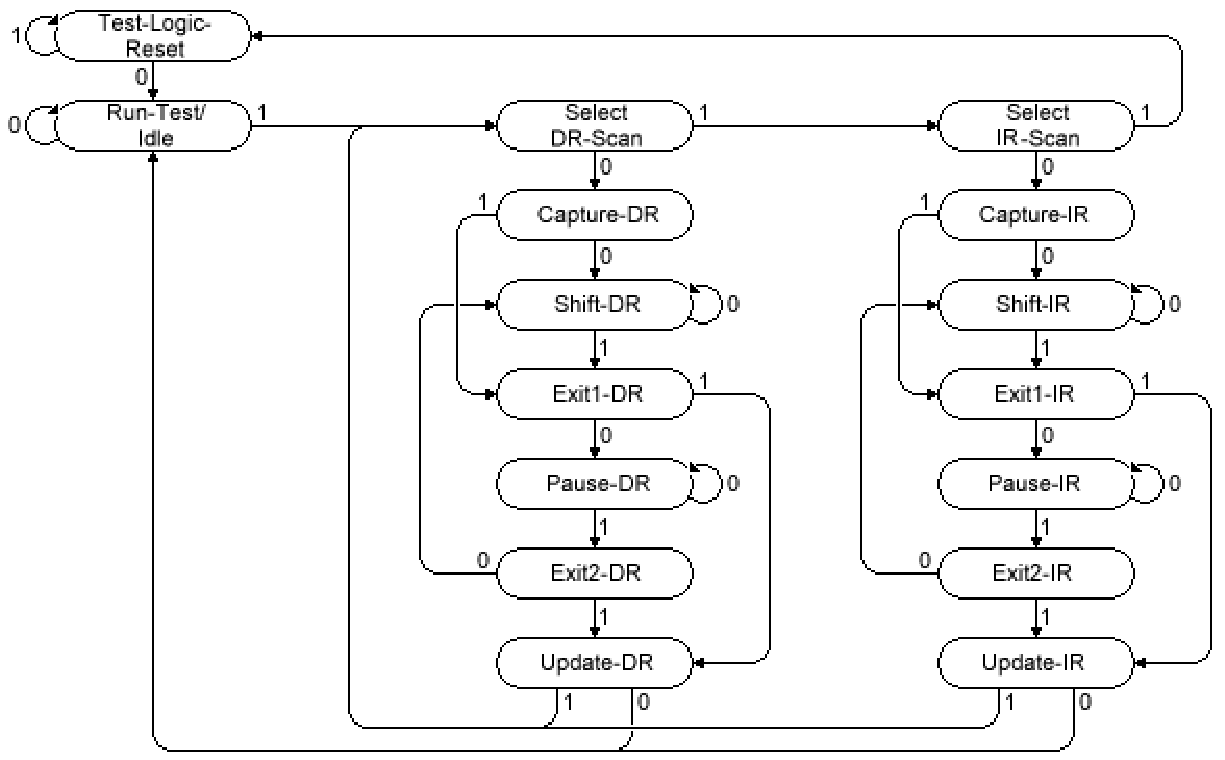
\includegraphics[width=0.47\textwidth]{figures/jtagsm}
	\centering
	\caption{JTAG TAP state machine.}
	\label{fig:jtagsm}
\end{figure}


The JTAG standard has four common registers: Instruction Register (IR) and Data Register (DR),  IDCODE, and BYPASS. The IDCODE register contains data that uses a standardized format that includes a manufacturer code. The BYPASS register is a single-bit data register that allows this device to be bypassed (do nothing) while other devices in the scan chain are examined. The IR and DR register's size depends on the TAP implementation, and they are used to send in instruction and receive result data.

The TAP implementation defines instructions and associated them with internal data registers. For instance, the host sends the IDCODE instruction through IR and subsequently gets the value of a 32-bit register (IDCODE) from TDO.

The PLC we used in this paper uses an ARM core microcontroller, namely, Texas Instruments Stellaris LM3S2793~\cite{lm3s2793}. The debug functionality provided in LM3S2793 is as CoreSight components. It provides real-time access for the debugger without halting the processor to AMBA (Advanced Microcontroller Bus Architecture)~\cite{flynn1997amba} system memory, peripheral registers, and all debug configuration registers. The TAP controller is implemented using CoreSight technologies, and it is called Debug Access Port (DAP) instead.

\begin{figure}[ht]
	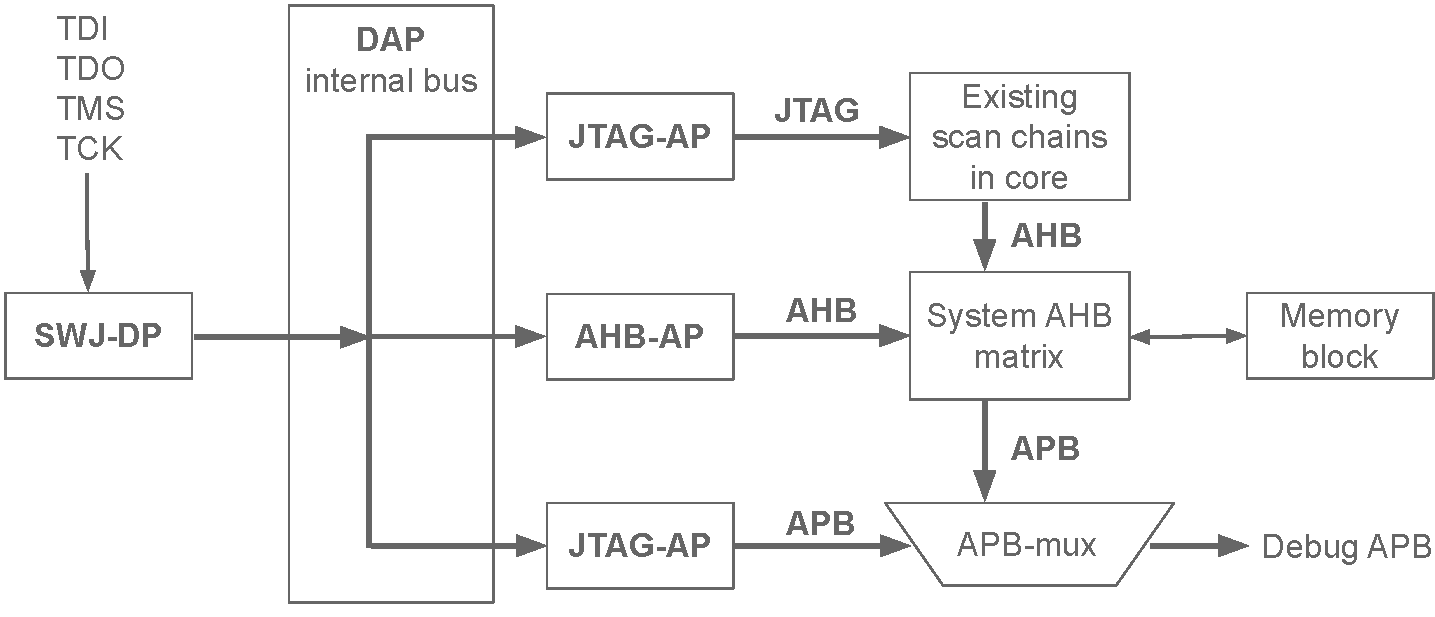
\includegraphics[width=0.47\textwidth]{figures/dap}
	\centering
	\caption{The debug port (DP) receives host signals and maintains the JTAG state machine. The instruction and data are sent to the DAP core through IR and DR, respectively. Unlike the JTAG standard that needs to halt the processor before reading registers, using CoreSight DAP, the registers, SARM, and MMIO can be accessed during runtime without halting the processor.}
	\label{fig:dap}
\end{figure}


As shown in~\autoref{fig:dap}, each DAP contains Debug Ports (DPs) and Access Ports (APs). The DP provides access to the DAP from an external debugger. Then the DAP uses the APs to access on-chip resources. Multiple APs such as AHP-AP, ABP-AP, and JTAG-AP respond to each type of bus and the devices that connect to it. For instance, the AHB-AP provides an AHB-Lite master for accessing the system AHB bus, which we use to access the RAM and MMIO.




%! TEX root = 'main.tex'
\section{Overview}
\label{sec:implant-overview}


%Critical infrastructure such as power grids comprises physical and cyber systems and assets that are vital to national security. Their failure or incapacity would have a significant impact on people's daily life on a large scale. The recent Ukrainian power grid attack, the massive blackout in south American countries~\cite{haes2019survey} demonstrated that influence not only affects people's livelihoods but even international politics. The cyberattack on the ICS system can even cause physical damage to the infrastructure~\cite{zeller2011myth}, which makes it harder to recover. Incidents such as the Stuxnet proved this point.

%Consequently, ICS has received considerable attention due to security concerns. There are many ways to breach a computer system, and most of them are focus on software-based approaches such as vulnerability hunting and exploiting, cracking of authentication and protocols. Therefore, the attacker needs to break into the network and avoid existing access control and other mitigations. Moreover, most critical infrastructures use their air-gapped network, and It may take a state-sponsored team to accomplish such as mission ~\cite{langner2011stuxnet}. 

%Under such circumstances, we believe that cyber-attacks with the assistance of physical approaches are underestimated, especially before the emergence of the so-called supply-chain attacks. Among those world-class attacks, the term APT(Advanced Persistent Threat) is often mentioned. In essence, the APT attack is an extremely well-hidden trojan that can be deployed for many years without being detected. Thus, installing the trojan and remotely triggering it is the crucial point of a successful attack.

In this paper, we present \name, an APT using a hardware implant that an attacker uses to perform coordinated distributed attacks on critical infrastructure such as power grid. To achieve this, we reversed engineered a PLC, developed a prototype of a hardware implant, and showed that such attacks could be performed even without state-sponsored attack groups. \name hijacks the data lines on the PLC and modifies them based on the command received by the attacker. Since the attacker can send such signals remotely, they can control various PLCs at different locations simultaneously to perform a coordinated distributed attack on the entire power grid.

\begin{figure*}[tp!]
	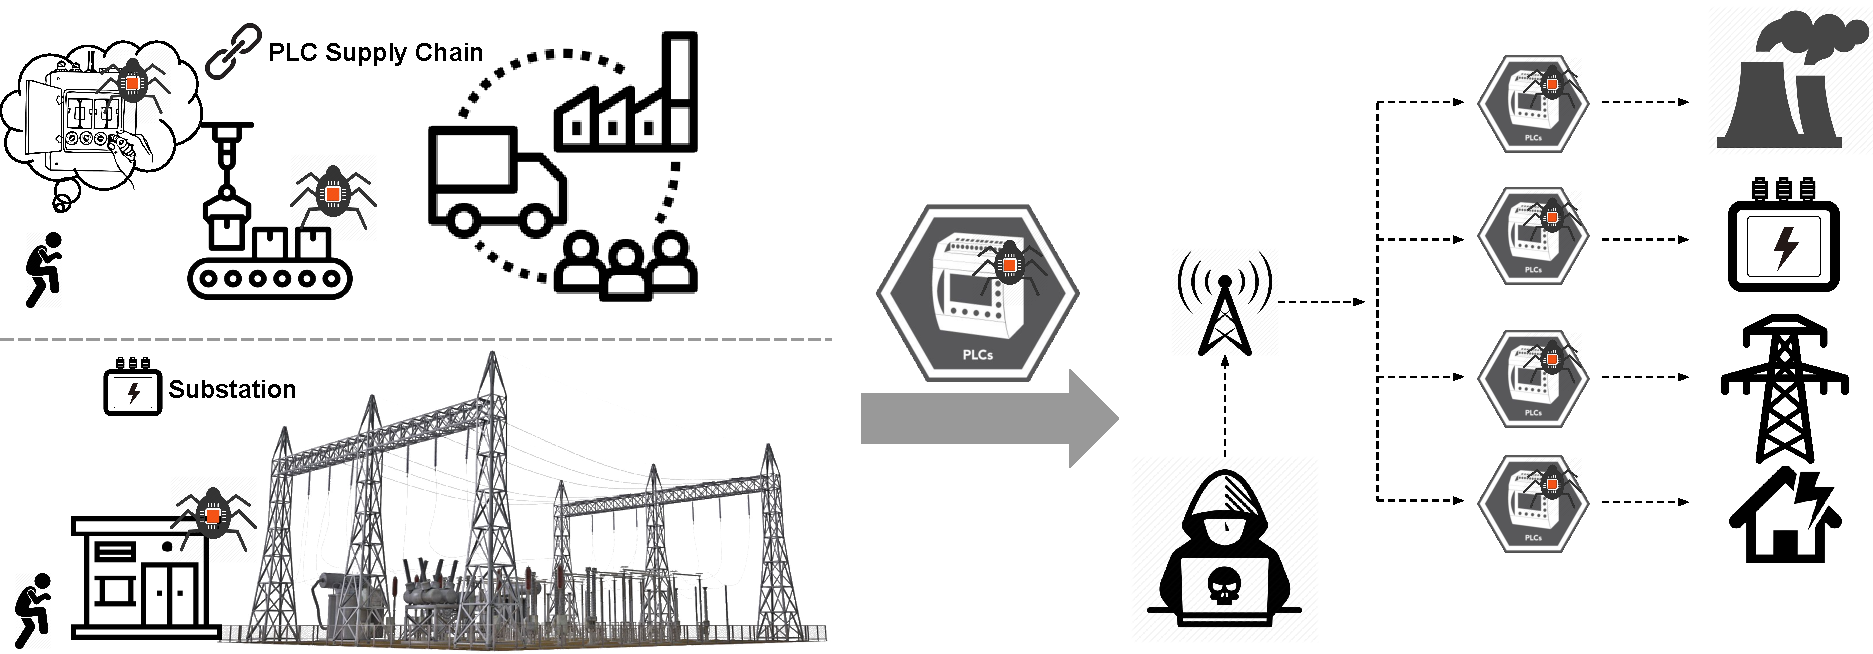
\includegraphics[width=\textwidth]{figures/bigpic}
	\centering
	\caption{In the PLC manufacturer factory or during the product shipment, numerous employees can access the PLCs. The hardware backdoor installation should follow specific procedures to be efficiently accomplished without advanced software knowledge. The hardware backdoor can communicate with the attacker through the GSM network. Therefore it does not need to join the ethernet used by the ICS system.}
	\label{fig:bigpic}
\end{figure*}

\name can be implanted into the PLC in two ways, including installing it during the supply chain or after the PLC has been deployed. These two scenarios are depicted in ~\autoref{fig:bigpic}. At first, during the supply chain, such as the factory and shipment, numerous employees can access the PLC. Installing an extra piece of a circuit board is not a difficult task for professionals~\cite{harrison2021malicious, o2015special}. Secondly, after the PLCs are being deployed, the power grid's vast distribution network lacks strong physical security \cite{Loopholes2020}. An attacker can sneak into one of the substations and install the hardware backdoor. The difficulty between the targeted PLC and the attacker, in reality, can be just a few padlocks. We believe that a substation's breach can cause a chain reaction in a power grid, and it is a real threat~\cite{substationattack, chen2020study}.

%In this paper, we provide two plans for physically installing a trojan and provide a prototype hardware implant \name that can be used for this type of attack. ~\autoref{fig:bigpic} depict the scenario. In many parts of the supply chain, such as the factory and shipment, numerous employees have the opportunity to access the PLC. Installing an extra piece of a circuit board is not a difficult task for professionals. Moreover, a large-scale infrastructure such as a power grid has many remote substations with very few staff. An attacker can sneak into one of the substations and install the hardware backdoor. The difficulty between the targeted PLC and the attacker, in reality, can be just a few padlocks. We believe that the breach of a substation can cause a chain reaction in a power grid, and it is a real threat~\cite{substationattack}~\cite{chen2020study}.


After the attacker controls enough PLCs, he can remotely initiate a distributed attack to cause more significant damage to the critical infrastructure using a cellular network. The advantage of this attack is that it does not rely on the existing ICS network, nor is it limited to the firmware running on PLCs so that it can evade most software-based mitigations. It only needs to know the specific PLC model of the target and modify the hardware implant accordingly.


\subsection{Adversary Model}

We assume that the attacker has physical access to the PLC once to implant the \name. Many studies and reports have shown that those attacks are not superficial and have been done in the real world during manufacturing or shipment~\cite{harrison2021malicious, o2015special, robertson2018big}. Since the attack is aware of the PLC model being targeted, we assume that the attacker knows the PLC's internal. The assumption could be made since the attacker can purchase a replica of PLC from any vendor. 

%The attacker knows the target's specific PLC model and can obtain the exact model for studying.

The printed circuit board (PCB) and the IC chips of the PLC should be well exposed. For example, the Chip-on-Board (COB)~\cite{lau1994chip} packing brings extra challenges for the attacker. The black glob-top makes it challenging to identify the chip model and pins. Fortunately, high-end microcontroller products rarely use this packaging. It would be a great advantage if the attacker can use the JTAG interface of the microcontroller. In other words, the JTAG interface is not disabled by programming fusing bits at the factory. Nevertheless, the attacker can control the IO or tamper with the firmware image when transferred through the bus without JTAG.

\name is less invasive than the firmware. Hence, there are no modifications to the operating system, the system software, or software mitigation solutions that run on a microcontroller. Hence, \name is undetected by such software mitigation solutions. The PLC system is allowed to have any memory protection mechanisms based on MMU~\cite{shalan2000dynamic} and MPU~\cite{kim2018securing}.

To remotely control the device, the attacker uses a GSM network or WIFI to communicate with the hardware backdoor. The PLC must not be deployed in an electromagnetic isolation environment (Faraday cage) where the wireless signal can not be transmitted outside. The assumptions are reasonable since many communications in such substations happen through wireless communications used by remote terminal units (RTUs).



\subsection{Challenges}

The major challenge in attacking PLCs is not having enough information about the device. Some vendors publish the microcontroller's datasheet, but some vendors use proprietary design with highly customized instruction set architecture (ISA).  The layout of the PCB board and the onboard pin definition are also not publicly available.


\textbf{\textit{Firmware.}} In an embedded system, flash memory usually stores a file system and a real-time operating system (RTOS) such as VxWorks~\cite{neugass1991vxworks}. It is the so-called firmware. Specific to a real-time microcontroller, the firmware runs bare-metally on the microcontroller or with a lightweight RTOS such as FreeRTOS~\cite{barry2008freertos}. Allen Bradley 1769-L18ER-BBIB CompactLogix 5370 has minimal information about the firmware being used. 

\textbf{\textit{Identifying Components on Board.}} Due to the lack of information and many proprietary chips used by such vendors, it is difficult to identify the chips used on the PLC board. Some of the chips have BGA packaging~\cite{joshi2000mosfet} where the pins are buried underneath. So it is difficult to trace the circuit board and identify the connections and pins such as JTAG. 

\textbf{\textit{Prototype.}} The main challenge of developing such an implant is power consumption. For reducing the footprint, a small chip had to be used that contains all the tools that could be used for hijacking, information retrieval, and modification of the signals. Not many tools are present for such a bare metal implant, and they have to be ported to work on a minimal computing base.   


%! TEX root = 'main.tex'
\section{Reverse Engineering and Design}
\label{sec:implant-design}


The major challenge in making a PLC-specific hardware backdoor is that PLC does not use open standards like PC.  During the development, a significant amount of time is spent on the reverse engineering of the PLC. After a basic understanding of its modules and chips, we can choose how to control it, whether through JTAG or intercepting other low-speed buses.


\subsection{Reverse Engineering}
The PLC we use is Allen-Bradley 1769-L18ER-BB1B/B CompactLogix 5370.
The reverse engineering work includes both the hardware and software parts. First, we speculate on the function of each board of the PLC. Then we identify the on-board IC chips and use a multimeter to conduct the connectivity test for wire tracing. The purpose of this is to find the interconnections between chips and between boards. Fortunately, the real-time module is a two-side PCB, and the wire connectors that pass through the board are well exposed, as seen in~\autoref{fig:ssi0}. Furthermore, we dump the firmware from the microcontroller and flash chip for reverse-engineering analysis.


\textbf{\textit{Backplanes.}} The Allen Bradley PLC contains several PCB module boards, known as backplanes. ~\autoref{fig:modules} shows each module. In this paper, we name the board with the Ethernet socket and USB port as the communication module (\textbf{B}).  The one controls that has a microcontroller and controls the 16 digital DC input pins and 16 digital DC output pins as the real-time module {\textbf{C}}, which is our main target. Module \textbf{D} is merely a connector for the digital IO. The rest are the power supply module(\textbf{A}) and LED module(\textbf{E}).


The communication module (\textbf{B}) itself is an embedded system, including a CPU, DRAM, and other peripherals such as Ethernet, SD card, and USB.  It communicates with the host (HMI) to receive firmware and ladder logic updates, and it also hosts a web server to display status. However, this module does not directly interact with IO. By analyzing the PLC firmware update files, we find that this board runs VxWorks operating system. Nevertheless, this board's primary chip is an FPGA~\cite{kuon2008fpga} chip that runs a soft-core ARM processor, and it is in BGA packaging. It is not easy to trace and identify which GPIO pins of the FPGA are used as the JTAG interface. We consider it as one of our further works. Therefore, our focus is the real-time module (\textbf{C}) that runs ladder logic and directly controls IO. Fortunately, this module uses a commercial microcontroller, namely, Texas Instruments Stellaris LM3S2793 SoC.

The digital IO sockets on the connector module (\textbf{D}) connects to the real-time module (\textbf{B}). The IO goes through the power switches and optically coupled isolator chips and eventually connects to the microcontroller, as shown in~\autoref{fig:board}. There are 32 LEDs corresponds to each IO socket, and the real-time module also controls the LED module through the I2C protocol. The power module (\textbf{A}) provides stable 3 volts for other boards. Our backdoor can either get power directly from it or the JTAG pad.

\begin{figure}[th]
	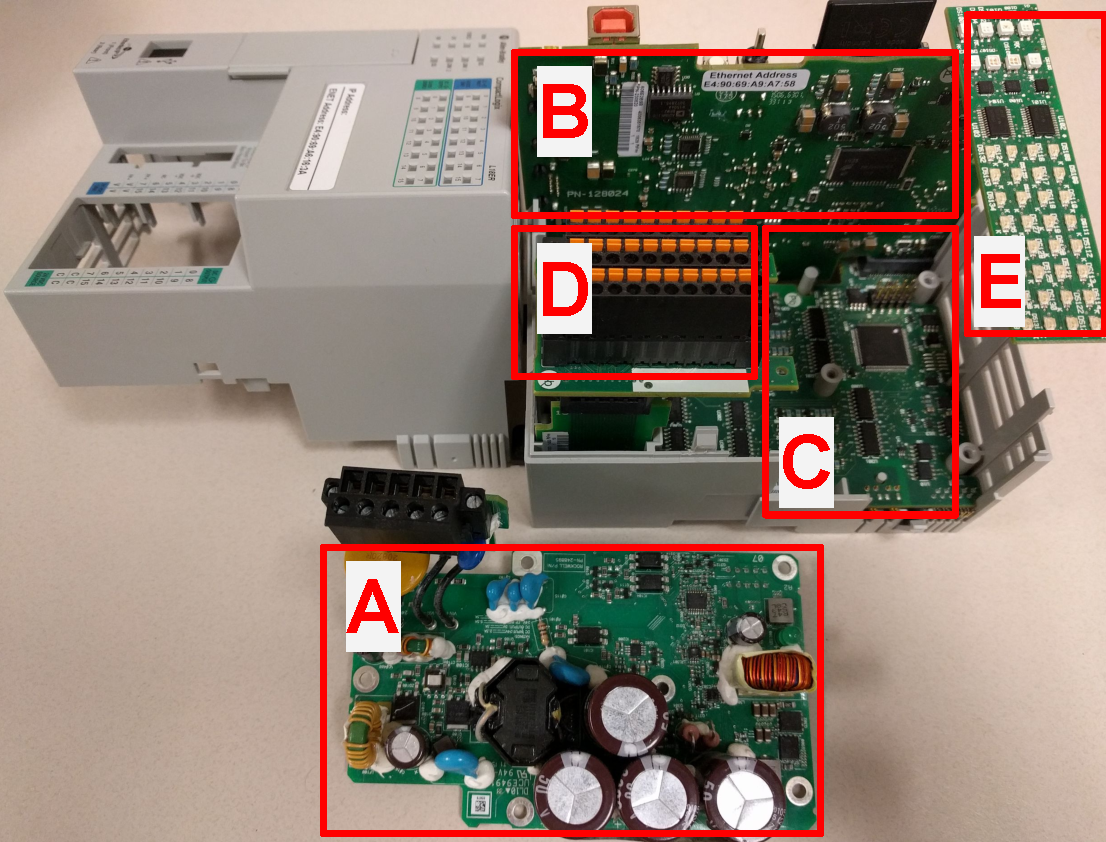
\includegraphics[width=0.47\textwidth]{figures/modules}
	\centering
	\caption{Allen-Bradley 1769-L18ER-BB1B/B CompactLogix 5370 PLC. A: Power supply module  B: Communication module  C: Real-time module  D: (16) DC Digital Outputs \& (16) DC Digital Inputs Connector  E: LED  module}
	\label{fig:modules}
\end{figure}




\textbf{\textit{Microcontroller.}} The TI Stellaris LM3S2793 SoC has an ARM Cortex-M3 processor core that operates at 80 MHz. It contains 64 KB SRAM and 128 KB flash. The internal ROM is preprogrammed with Stellaris Peripheral Driver Library (DriverLib) to drive the on-chip peripheral devices. ~\autoref{tab:memorymap} shows the memory map. 


\begin{center}
	\begin{table}
		\small
		\begin{tabular}{p{1.6cm}  p{1.6cm}  p{4cm}} 
			\hline
			%Start & End & Description \\ [0.5ex] 
			Start & End & Description \\ 
			\hline
			\multicolumn{3}{l}{\textbf{Memory} (0x00000000 - 0x22200000)}  \\
			\hline
			0x00000000 & 0x0001FFFF & On-chip Flash \\ 
			\hline
			0x00020000 & 0x00FFFFFF & Reserved \\
			\hline
			0x01000000 & 0x01004FFF & On-chip ROM  \\
			\hline
			0x01005000 & 0x01005EFF & AES+CRC lib in on-chip ROM   \\
			\hline
			... & & \\
			\hline
			%0x01005F00 & 0x1FFFFFFF & Reserved \\ 
			%\hline
			0x20000000 & 0x2000FFFF & Bit-banded on-chip SRAM \\
			\hline
			... & & \\
			\hline
			%0x20010000 & 0x21FFFFFF & Reserved \\
			%\hline
			%0x22000000 & 0x221FFFFF & Bit-band alias of bit-banded on-chip SRAM starting at 0x20000000 \\
			%\hline
			%0x22200000 & 0x3FFFFFFF & Reserved \\
			\multicolumn{3}{l}{\textbf{FiRM Peripherals} (0x40000000 - 0x4001FFFF)}  \\
			\hline
			... & & \\
			\hline
			0x40008000 & 0x40008FFF & SSI0 \\
			\hline
			... & & \\
			\hline
			\multicolumn{3}{l}{\textbf{Peripherals} (0x40020000 - 0xDFFFFFFF)}  \\
			\hline
			0x40020000 & 0x400207FF & I2C Master 0 \\
			\hline
			... & & \\
			\hline
			0x4005C000 & 0x4005CFFF & GPIO Port E (AHB aperture) \\
			\hline
			0x4005D000 & 0x4005DFFF & GPIO Port F (AHB aperture) \\
			\hline
			0x4005E000 & 0x4005EFFF & GPIO Port G (AHB aperture) \\
			\hline
			0x4005F000 & 0x4005FFFF & GPIO Port H (AHB aperture) \\
			\hline
			... & & \\
			\hline
			\multicolumn{3}{l}{\textbf{Private Peripheral Bus} (0xE0000000 - 0xFFFFFFFF)}  \\
			\hline
			... & & \\
			\hline
			0xE000E000 & 0xE000EFFF & Nested Vectored Interrupt Controller (NVIC) \\
			\hline
			... & & \\
			\hline
		\end{tabular}
		\caption{LM3S2793 Memory Map. Only list the address space of the memory and devices related to this paper. FiRM-compliant (compliant to the ARM Foundation IP for Real-Time Microcontrollers specification).}
		\label{tab:memorymap}
	\end{table}
\end{center}


\textbf{\textit{Reset Vector.}} The vector table is at a fixed address 0x00000000 after the system reset. The core starts to execute from memory 0x00000004, which is the reset vector. ~\autoref{tab:memorymap} shows that the reset vector resides in the flash memory instead of the ROM. It is because the ROM boot loader is only executed in two scenarios. The first case is when the flash memory is empty. The other one is when an application initiates a firmware update and calls the ROM boot loader to execute. For instance, if data at 0x00000004 is 0xFFFFFFFF, which indicates an empty flash, then the ROM is mapped to 0x00000000 to substitute the flash and execute instead. 

The data at 0x00000000 and 0x00000004 will be loaded into the stack pointer (SP) and the program counter (PC), respectively. In our case, the SP is 0x20000B48, and the PC is 0x000000E3. Notice that 0xE3 is an odd number. As we know, RISC processors such as ARM uses fixed-length instruction. On ARM processors, setting the PC's least significant bit indicates that the following code will be executed as the two-byte Thumb instructions. Therefore, we dump the flash memory and disassemble it at address 0x000000E2 instead.



\textbf{\textit{Flash Boot Loader.}} Right after the flash boot loader starts, it copies itself to SRAM, starting at 0x20000000. Although both SRAM and flash memory can be accessed in a single cycle, flash memory can do that as long as the code is linear and branches incur a one-cycle stall. The bootloader copies 0x00000000 - 0x00000A88 to 0x20000000 - 0x20000A88, and clear the data section (0x20000A88 - 0x20000F54). As mentioned earlier, on system reset, the vector table is at the fixed address 0x00000000. However, it can be relocated by writing the vector table offset register (VTOR:0xE000ED08). Changing the vector table indicates a complete change of the system's behavior because all the interrupt handlers are new, and they interpret how the system behaves regarding peripheral device's requests. The bootloader sets the vector table to 0x20000000 and jumps back to SRAM to continue execution.


\textbf{\textit{Stellaris Peripheral Driver Library.}} The Drivelib~\cite{lm3s2793rom} is a set of APIs utilized to control the on-chip peripheral devices. It is provided in ROM code and placed in a fixed location on Cortex-M3 SoCs. It helps identify what functions the firmware calls. Through the fixed location of APIs and the Drivelib datasheet, the function matches with names. It is a two-level table structure. The main table is at 0x1000010, and it contains the address of the second-level table for each type of peripherals, as shown in~\autoref{tab:romtable}. For example, ~\autoref{tab:gpiotable} shows the \texttt{ROM\_GPIOTABLE}, which contains all the GPIO related APIs.

\begin{center}
	\begin{table}
		\small
		\begin{tabular}{|p{7.2cm}|} 
			\hline
			\texttt{ROM\_APITABLE (0x1000010)} \\ %[0.5ex] 
			\hline
			[0] = \texttt{ROM\_VERSION} \\
			\hline
			[1] = pointer to \texttt{ROM\_UARTTABLE} \\
			\hline
			[2] = pointer to \texttt{ROM\_SSITABLE} \\
			\hline
			[3] = pointer to \texttt{ROM\_I2CTABLE} \\
			\hline
			[4] = pointer to \texttt{ROM\_GPIOTABLE} \\
			\hline
			[5] = pointer to \texttt{ROM\_ADCTABLE} \\
			\hline
			... \\ 
			\hline
		\end{tabular}
		\caption{LM3S2793 ROM API table is at a fixed address 0x1000010, and each table entry is 4 bytes address that points to a second-level table, which corresponds to a class of peripheral devices.}
		\label{tab:romtable}
	\end{table}
\end{center}

\begin{center}
	\begin{table}
		\small
		\begin{tabular}{|p{7.2cm}|} 
			\hline
			\texttt{ROM\_GPIOTABLE} \\ %[0.5ex] 
			\hline
			[0] = function \texttt{ROM\_GPIOPinWrite} \\
			\hline
			[1] = function \texttt{ROM\_GPIODirModeSet} \\
			\hline
			[2] = function \texttt{ROM\_GPIODirModeGet} \\
			\hline
			[3] = function \texttt{ROM\_GPIOIntTypeSet} \\
			\hline
			[4] = function \texttt{ROM\_GPIOIntTypeGet} \\
			\hline
%			[5] = function ROM\_GPIOPadConfigSet \\
%			\hline
			... \\ 
			\hline
		\end{tabular}
		\caption{GPIO API Table. Each table entry is the entry address of an API, and the function parameters are passed through registers. There is no privilege or mode change when calling into the APIs.}
		\label{tab:gpiotable}
	\end{table}
\end{center}



\autoref{fig:romapiexample} shows a typical code snippet that calls a ROM API. The second-level table is at 0x1000010 + 0x10 (\texttt{ROM\_APITABLE[4]}), which is the the GPIO table. And the API it calls is \texttt{ROM\_GPIOPinRead()} (\texttt{ROM\_GPIOTABLE[11]}). Because all the ROM API call sites have the same pattern, it makes firmware's reverse engineering work much easier.  Calling the API is merely locating the function address from the two-level tables and jumps to it, and the parameters are passed in through registers. There is no privilege change when calling into the APIs, and the firmware code all runs in the system mode.


\begin{figure}[th]
	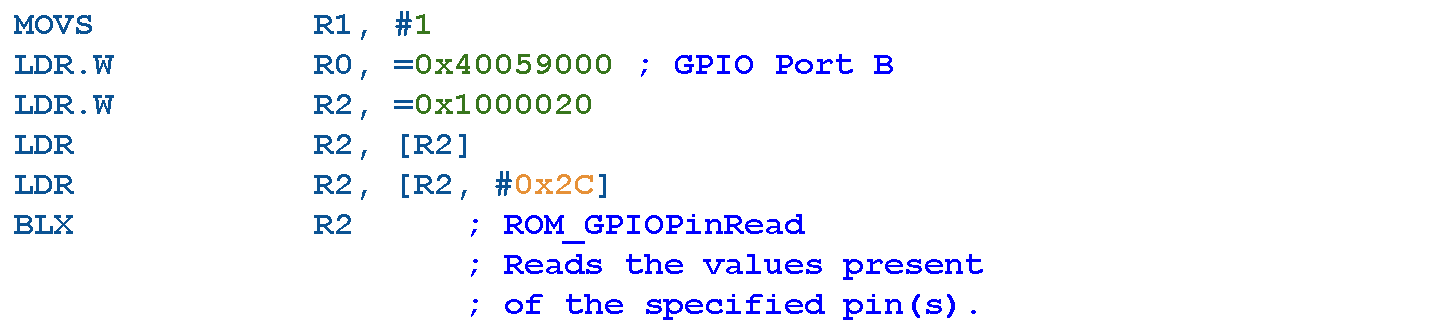
\includegraphics[width=0.47\textwidth]{figures/romapiexample2}
	\centering
	\caption{A code snippet that calls \texttt{ROM\_GPIOPinRead()}. The parameters are passed through registers. In this case, the  \texttt{ROM\_GPIOPinRead()} has two parameters. R0 contains the GPIO port address, and R1 indicates the pins to operate.}
	\label{fig:romapiexample}
\end{figure}




%\textbf{\textit{Debug.}} In addition to reverse-engineering,  we also need to debug the firmware. We use the SEGGER J-Link debugger. Since the target is ARM and the debugger sets up a GDB server, we also need GNU Embedded Toolchain for ARM~\cite{gnutoolchainarm}, an ARM version of the gdb client.
%
%
%As mentioned earlier, the stack pointer and program counter are located at address 0x00000000 and 0x00000004. As shown in~\autoref{fig:gdbinit}, we use a GDB initialization script that contains GDB commands to set up the target. This script makes the PLC initialized and runs ladder logic, but the PLC cannot be interrupted during runtime with the debugger. If so, the indicator on the LED panel will prompt an IO error. The reason is still under investigation, and it could be that the watchdog timer is not handled well.
%
%\begin{figure}[th]
%	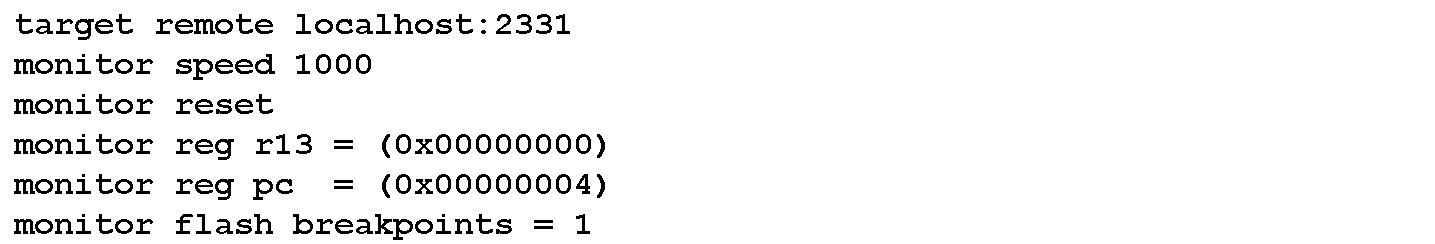
\includegraphics[width=0.47\textwidth]{figures/gdbinit}
%	\centering
%	\caption{The minimal gdbinit script that sets the SP and PC registers makes the PLC be up and running. Other on-chip peripheral controllers may not be correctly initialized.}
%	\label{fig:gdbinit}
%\end{figure}
%


%\subsubsection{more reverse engineering topics ....}

%Through reverse engineering, it shows that the Vector Table Offset Register is first at address 0x0, then switch to address 0x20000000, after receiving the ladder logic code, finally set to address 0x40000. 



\textbf{\texttt{GPIO.}} The PLC interacts with the physical world through digital inputs and outputs. The IO goes through the power switches and optically coupled isolator chips and eventually connects to the microcontroller's GPIO.


In the microcontroller LM3S2793, the GPIO module comprises nine physical GPIO blocks, and each corresponds to an individual GPIO port. Depending on the microcontroller's configuration, it supports up to 67 programmable input/output pins or several pins grouped to provide peripheral functions such as I2C. The GPIO ports can be accessed either through AHB or APB bus, which matters when we access the GPIOs through JTAG. We choose the AHB-AP.

Each GPIO port has several associated control registers, such as GPIO Digital Enable (GPIODEN), GPIO Alternate Function Select (GPIOAFSEL), GPIO Port Control (GPIOPCTL), and GPIO Data Control registers. All GPIO pins are configured as individual input/output pins and tri-stated by default. The GPIO Direction (GPIODIR) register configures each GPIO pin as an input or output, and we do not change it. To change the inputs and outputs, we primarily operate on the GPIO Data (GPIODATA) register that modifies individual bits in GPIO ports. 

The way to control the GPIO data is not straightforward.  Different microcontrollers adopt different operating methods. For example, the GPIO port may take Output Data Register (ODR), Bit Reset Register (BRR), Bit Set/Reset Register (BSRR)~\cite{cottle2001programmable}. In our case, the LM3S2793 microcontroller uses a more complicated model to conduct bit-wise operations. The GPIO Data register is memory-mapped. When read/write, bits[9:2] of the address are treated as a bitmask, as well as the bits[1:0] are always zero because the memory access should be at 4-byte alignment on ARM. Therefore, for each GPIO port, the memory-mapped range should be 1KB long, that is, from GPIODATA to GPIODATA + 0x3FC. A write can only change the data bit when the corresponded bitmask is set. Otherwise, the data bit is unchangeable.

For example, GPIO Port A (AHB) is mapped at 0x40058000, and it controls 8 GPIO pins. We want to set bit2 to 0 and bit5 to 1. As shown in~\autoref{fig:gpiowrite}, the bitmask is 0x90, and the data is 0xF0.  Hence, the operation should be writing 0xF0 to address 0x40058090.


\begin{figure}[th]
	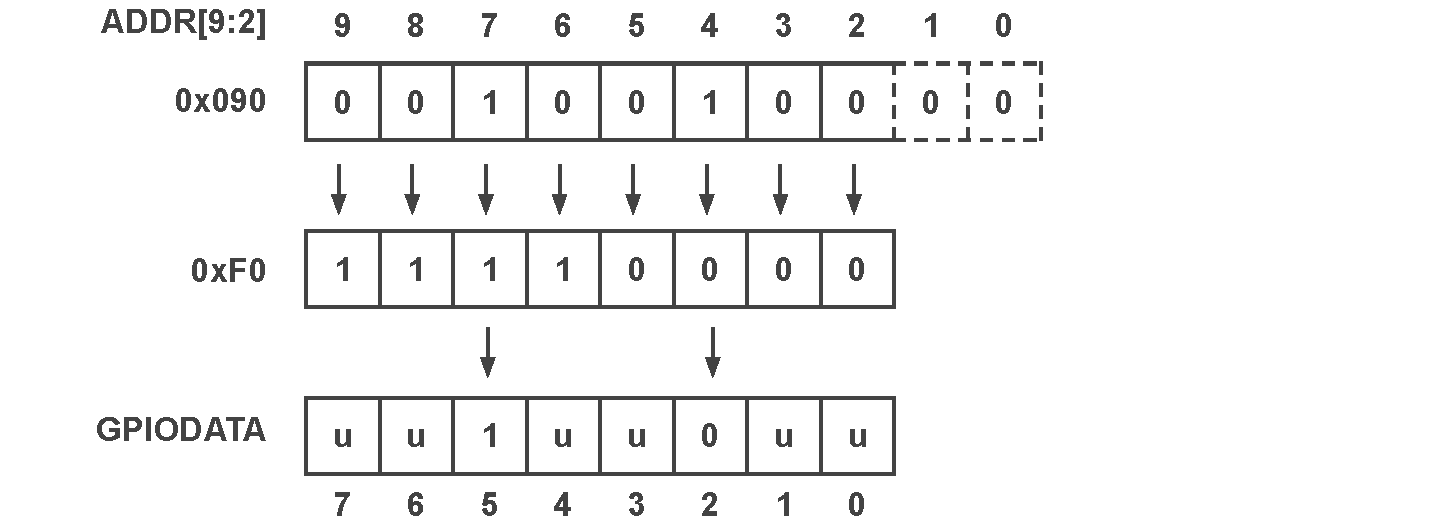
\includegraphics[width=0.47\textwidth]{figures/gpiowrite2}
	\centering
	\caption{Writing a byte of 0xF0 to address GPIODATA + 0x90.  The bitmask only allows bit2 and bit5 to be modified. Therefore, only two bits are valid for the write operation.  \textbf{u} indicates the new bit is ignored.}
	\label{fig:gpiowrite}
\end{figure}



The same applies to reading. Only the corresponding bit in the bitmask will be read. Otherwise, it reads zero. For example, to read the four high bits from GPIO Port A, the address with bitmask should be 0x40058000 + 0x3C0, and it reads 0xA0, as shown in~\autoref{fig:gpioread}.

\begin{figure}[th]
	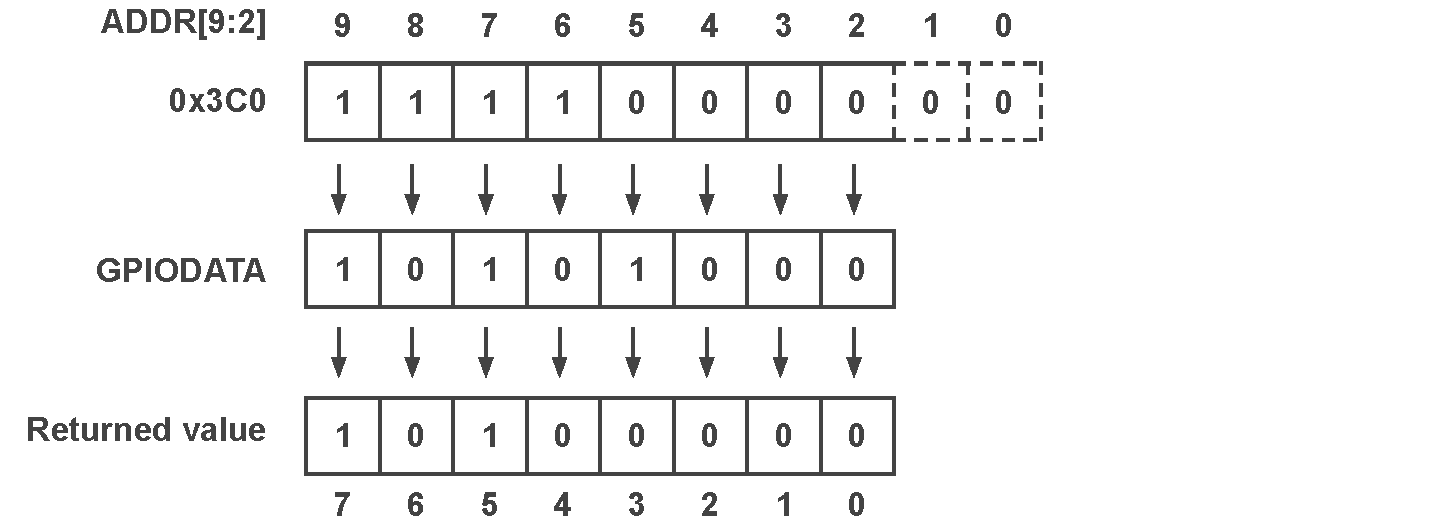
\includegraphics[width=0.47\textwidth]{figures/gpioread2}
	\centering
	\caption{The address GPIODATA+0x3C0 reads the high four bits of the GPIO port. The rest reads zero regardless of the actual value.}
	\label{fig:gpioread}
\end{figure}



\textbf{\texttt{Control Output.}} After knowing how to control GPIO, we can directly control the output of the PLC. There are 16 inputs and 16 outputs on the IO connector. Through reverse engineering, we know the GPIO port corresponding to the IO.  That are, GPIO port E (0x4005C000) GPIO port F (0x4005D000) for inputs, and GPIO port G (0x4005E000), GPIO port H (0x4005F000) for outputs. Intuitively, each GPIO bit corresponds to a pin on the connector. One indicates the high voltage, which is the field power voltage; zero dictates the low voltage (8 volts).

To conduct a stealthy attack, we want to change the output secretly. For example, we want to keep the LEDs in their original state and the host (HMI) not to find any abnormalities. To achieve this goal, we need to leverage the firmware itself. The PLC periodically scans the inputs, runs ladder logic, and updates outputs.  It is trivial to find the ladder logic binary by following the timer handler routine. There are a few local variables that control how the ladder logic behaves. For example, one local variable determines if any logic state has changed. If so, the corresponded GPIO pin will be updated according to the ladder logic. We modify this local variable so that everything looks up to date. In the meantime,  we can change the outputs without triggering any alarms.



\textbf{\textit{AT45DB021E SPI Flash Memory.}}  It is quite noticeable that right next to the LM3S2793 microcontroller,  there is an 8-pin flash chip, which is an Adesto 45DB021E 2-Mbit SPI flash memory. It connects with the PLC's SSI0 (Synchronous Serial Interface), as shown in ~\autoref{fig:ssi0}.

\begin{figure}[th]
	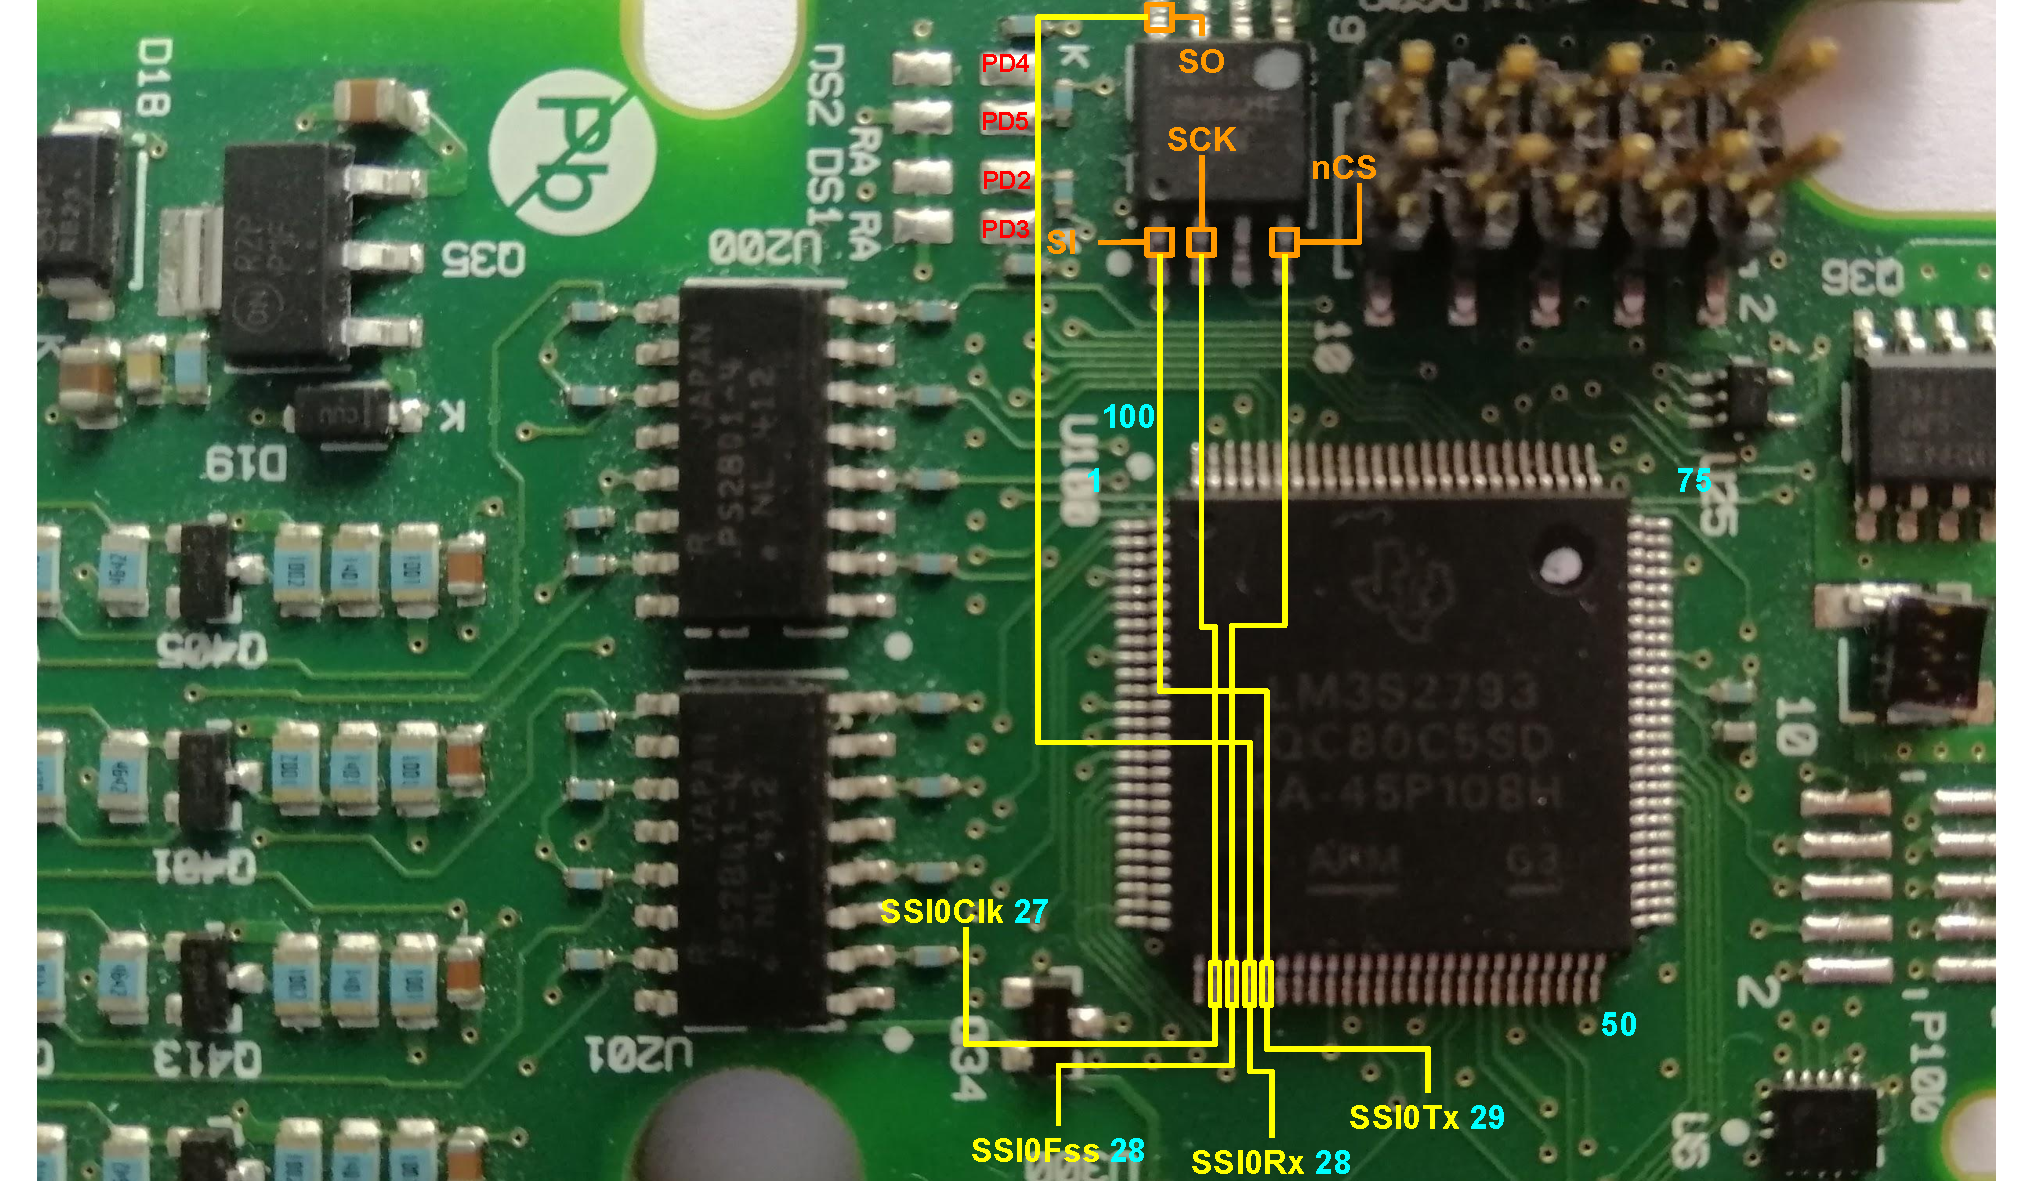
\includegraphics[width=0.47\textwidth]{figures/ssi0}
	\centering
	\caption{Through wiring tracing, we find that the AT45DB21E SPI Flash Memory connects to LM3S2793's SSI0 interface. The eight solder joints on the left may be used to install four LEDs. They are controlled by GPIO port D,  but they are not installed.}
	\label{fig:ssi0}
\end{figure}


During the boot process, the pins in GPIO port A are assigned for the SSI0 master device. The firmware first reads one byte from the flash chip (offset 0x2000), which looks like a status byte. If it equals 0x55 or 0xAA, the PLC will be reset. If not, the firmware checks the integrity of the address 0x4000 to 0x1FFFC, the compiled ladder logic. The algorithm is a simple checksum. Accumulate each byte in this address range, and the result should be equal to the byte in address 0x1FFFF.

So this status byte at 0x2000 indicates the status of the PLC last time it was running. The value 0x55 indicates that the system has encountered a severe failure. If so, the firmware operates on GPIO port D, leading to the eight solder joins next to the SPI flash. We think they may be four LEDs to show the status. Furthermore, if the value is 0xAA, it means that the ladder logic binary has been broken, and the firmware will copy the code from 0x6100 in the SPI flash. We think this is a backup code and also a place where malicious code can be stored.

To read the AT45DB21E flash chip's content, we port its driver to the Teensy 3.2 board. The source code is available at the github~\footnote{https://github.com/whensungoesdown/at45db021\_teensy32}.



\textbf{\textit{Front Panel LED.}} There are four rows of LEDs on the front panel of the PLC. Each LED represents the state of an input or output. Usually, this is a very intuitive reflection of the current status of the PLC.

There are four rows of LED lights on the PLC's front panel. Each LED shows individual input and output pins' status, which is an intuitive way for the administrator to check whether the device works properly. The microcontroller controls these LEDs through the I2C protocol~\cite{semiconductors2000i2c}.

There are two 24-pin PD9535 chips (Remote 16-bit I2C/SMBus, Low-Power I/O Expander~\cite{pd9535}) on module \textbf{E}. It provides general-purpose I/O expansion for microcontrollers via the I2C bus. The two pins in GPIO port B(PB2 and PB3) on the microcontroller are used as the SCL and SDA signal lines for the I2C master device. These two signal lines also pass through the connector between module \textbf{B} and \textbf{C}, as shown in~\autoref{fig:p607}.

Each I2C slave device on the same bus has a unique 7-bit address. In our example, the addresses of the two PD9593 chips are 0x20 and 0x21. ~\autoref{tab:i2ccommand} shows that the chip has eight internal registers. As mentioned in~\autoref{sec:implant-background}, after the master device successfully sends the address byte, it will send another byte to select the internal register. Among these internal registers, the configuration register is responsible for controlling the directions of the IO pins. Zero means the corresponding pin is output. Because the PLC uses PD9593 to control the LED, all the pins are outputs. The input port registers reflect the pins' incoming logic levels, regardless of whether the pin is defined as an input or an output by the configuration register. Nevertheless, we do not need to read the input registers.



\begin{center}
	\begin{table}
		%\begin{tabular}{|c|@{}c@{}|c|c|} 
		\begin{tabular}{|@{}>{\centering\arraybackslash}m{0.9cm}@{}|
				@{}>{\centering\arraybackslash}m{3.65cm}@{}|
				@{}>{\centering\arraybackslash}m{2.52cm}@{}|
				@{}>{\centering\arraybackslash}m{1.62cm}@{}| }
			\hline
			\makecell{CMD \\Byte} & Register & Protocol & \makecell{Power-up \\Default}\\
			\hline
			0x00 & Input Port 0 & Read byte & xxxx xxxx\\ 
			\hline
			0x01 & Input Port 1 & Read byte & xxxx xxxx\\
			\hline
			0x02 & Output Port 0 & Read/Write byte & 1111 1111\\
			\hline
			0x03 & Output Port 1 & Read/Write byte & 1111 1111\\
			\hline
			0x04 & Polarity Inversion Port 0 & Read/Write byte & 0000 0000\\
			\hline
			0x05 & Polarity Inversion Port 1 & Read/Write byte & 0000 0000\\
			\hline
			0x06 & Configuration Port 0 & Read/Write byte & 1111 1111\\
			\hline
			0x07 & Configuration Port 1 & Read/Write byte & 1111 1111\\
			\hline
		\end{tabular}
		\caption{The internal registers of the PD9593 are selected by the master device sending the command byte. To control the LED, we need to operate the control register and the output register and keep the two polarity inversion registers' default value.}
		\label{tab:i2ccommand}
	\end{table}
\end{center}


\autoref{fig:ledi2cinit} shows the pseudo-code to initialize the I2C IO expander using the ROM API. It first enables the I2C master device and sets the clock frequency to be the same as the microcontroller. After that, call \texttt{ROM\_I2CMasterSlaveAddrSet()} to select the target device's address, whether to send or receive data. Then call \texttt{ROM\_I2CMasterDataPut()} to set the data to be sent next. Only after calling \texttt{ROM\_I2CMasterControl()}, the data will be sent out. In our example, two bytes with content zero are sent to Configuration Port0 and Port1. This operation sets a total of 16 pins as output mode.



\begin{figure}[th]
	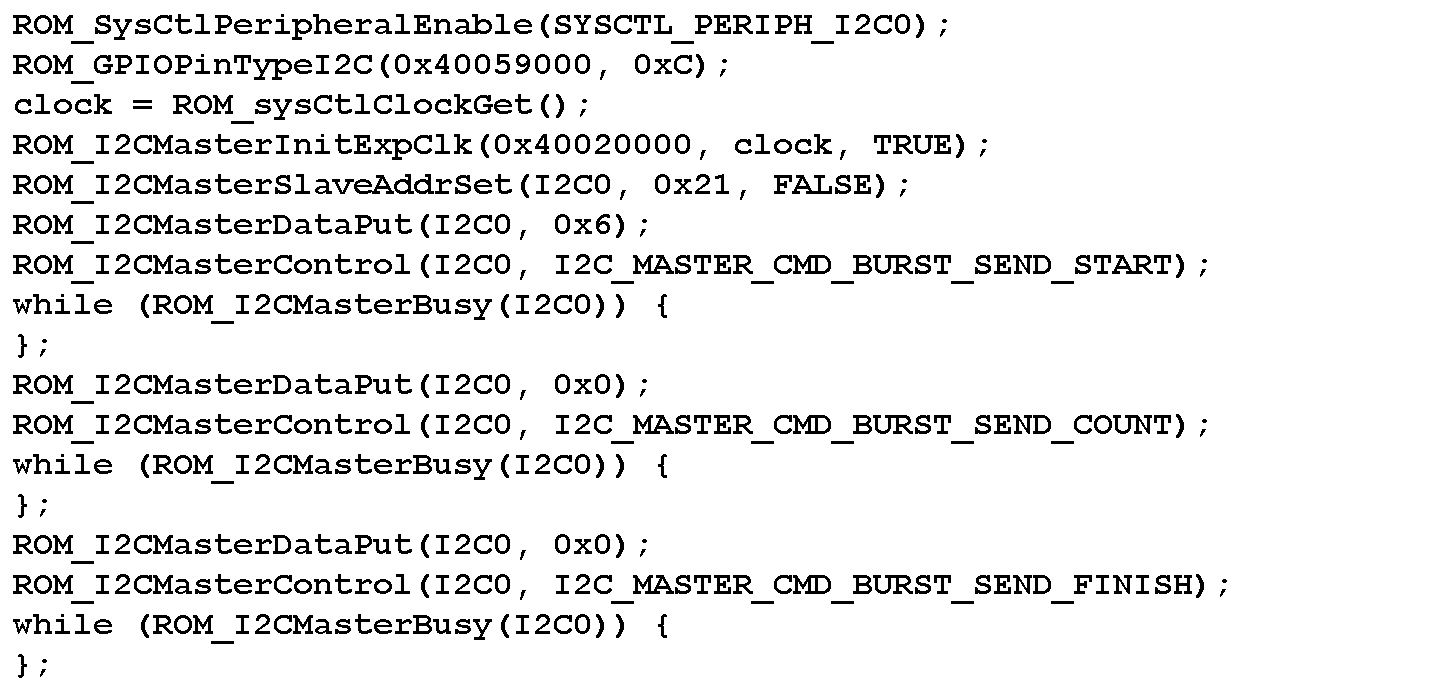
\includegraphics[width=0.47\textwidth]{figures/ledi2cinit}
	\centering
	\caption{The pseudo-code to initialize the I2C IO expander is reversed-engineered from the firmware. To make it more intuitive, we use some macro definitions as parameters. These macros' actual value is not difficult to find in the header files released by the vendor. The code is provided to help understand how to control the LED lights on the PLC through the I2C bus.}
	\label{fig:ledi2cinit}
\end{figure}



After initialization, \autoref{fig:ledi2csend} shows how to control the LEDs. For example, we send two bytes with content 0xFF to the Output Port0 and Port1, lighting up 16 LED lights controlled by this device.


\begin{figure}[th]
	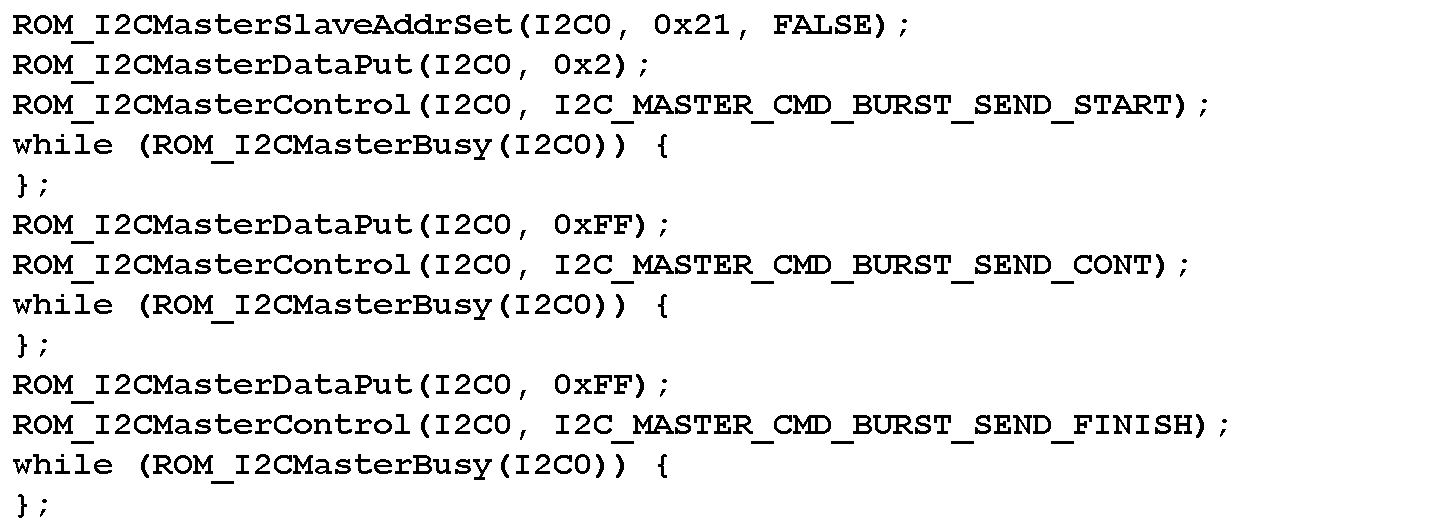
\includegraphics[width=0.47\textwidth]{figures/ledi2csend}
	\centering
	\caption{Each pin in the Output register controls an LED light separately, so two 0xFF bytes can control 16 LEDs. If we only want to control a few of the LED lights in one register, we can call \texttt{ROM\_I2CMasterControl() }with parameter \texttt{I2C\_MASTER\_CMD\_SINGLE\_SEND}.}
	\label{fig:ledi2csend}
\end{figure}






\textbf{\textit{Onboard Connectors.}} There are several connectors on the real-time module \textbf{C}, as shown in ~\autoref{fig:board}. P607 connects to the communication module \textbf{B} and P609 connects to the power module \textbf{A}. Usually, we think that the module \textbf{A} is just a power module responsible for providing three volts to others. However, this is a good place for purposefully damage the PLC by a short circuit, where the power flow is large.

By conducting the connectivity tests with a multimeter, we perceive some pins' function in P607 as shown in~\autoref{fig:p607}. As mentioned earlier, the I2C bus passes through this connector. Besides, the CAN bus also passes through this connector. In this way, both the communication module and the real-time module are connected to the CAN bus connector in the bottom right corner in ~\autoref{fig:board}. These two modules can not only control the external CAN bus device, but they can also communicate via the CAN bus themself. However, the communication module has a higher priority. Setting pin29 on the P607 connector can block the transmission of the signal on pin21, the CAN bus's RxD signal line. On the microcontroller side, the master device CAN0 uses the PA6 and PA7 pins. 


\begin{figure}[th]
	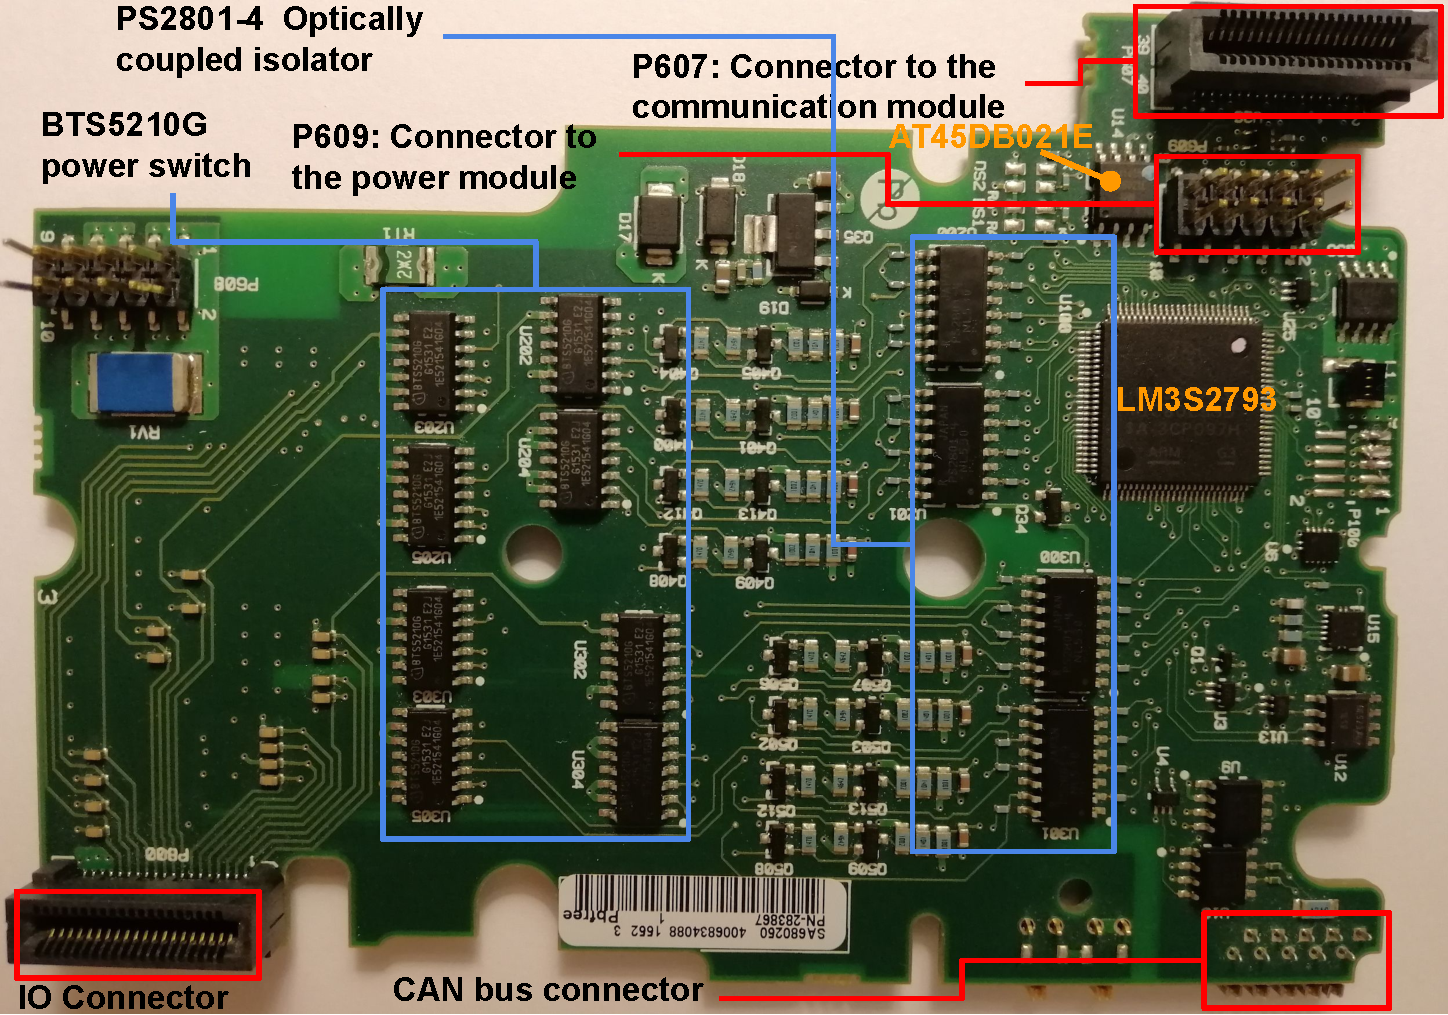
\includegraphics[width=0.47\textwidth]{figures/board3}
	\centering
	\caption{The real-time module reads the input signals, runs the ladder logic, and then drives the output signal according to the result. Therefore this module needs to be connected to all other modules. In addition to the microcontroller and the flash memory, there are power regulators and IO chips on this module. The optically coupled isolators prevent high voltages from affecting the microcontroller when receiving the signal, and the power switches provide the electrical connection between the output pin and the voltage source.}
	\label{fig:board}
\end{figure}


\begin{figure}[th]
	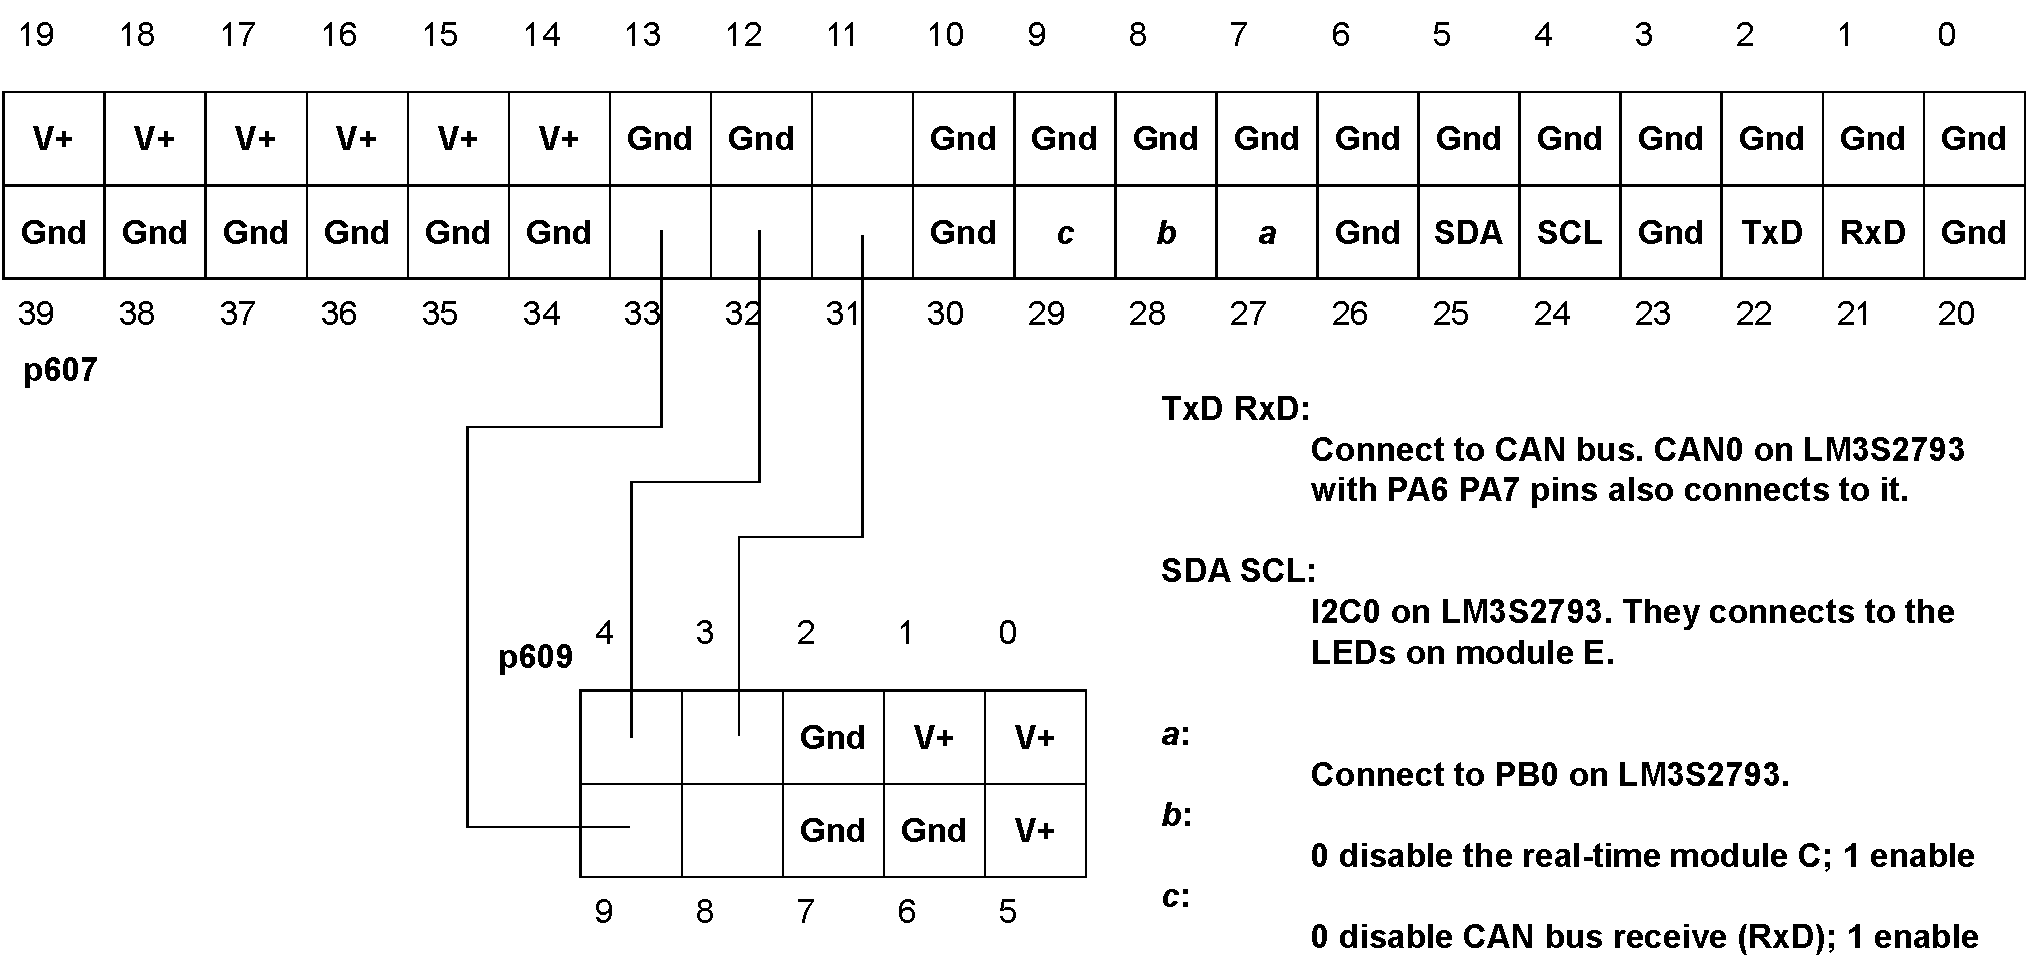
\includegraphics[width=0.47\textwidth]{figures/p607-2}
	\centering
	\caption{The connector between the communication board (module \textbf{B}) and real-time board (module \textbf{C}).  There are many pins, but the majority of them are power and ground. The microcontroller controls the LED module through the P607 connector.  The communication module can block the operation of the entire real-time module through pin28. However, there are still a few pins that we have not figured out their functions. We consider it as one of our further works.}
	\label{fig:p607}
\end{figure}

%As mentioned earlier, on module C, there is a AT45DB21E flash chip. It connects to the microcontroller through SSI0. And it contains one copy of code that will be loaded in once the microcontroller is caught in an unrecoverable error. But by analyzing this interface, we found that the communication module B is not connected to this AT45DB21E flash chip. So we think the code in it is just the backup code used to recover from the fatal error state, and the updated compiled ladder logic is updated by other means.  
%
%By reverse engineering the circuit board and firmware, we identified pin 24 and pin 25 of the connector as the SCL and SDA pin of I2C bus, as shown in~\autoref{fig:p607}. The microcontroller LM3S2793's PAxx PAxx connects LED module E through the communication module B, as shown in~\autoref{fig:modules}.
%
%We also identified that pin 21 and pin 22 are used as CAN bus input and output that come from the communication module B. And pin 29 is used to disable the CAN bus receive signal (RxD). On the CompactLogix PLC 1766, there is only one set of CAN bus for connecting modules. It located on the side of the PLC, it's part of the real-time module, as shown in~\autoref{fig:board}.
%
%
%Both the communication module B and real-time module C are connected to this bus.


\subsection{Design}

Typically, the PLC has a dedicated real-time microcontroller
that handles IO, in this case, module \textbf{D}. It runs minimal code, mainly the compiled ladder logic.  To receive ladder logic update, the communication module \textbf{C} talks to the HMI and then update the real-time microcontroller through the CAN bus. Therefore, to remotely control the PLC's IO, the attacker needs to control further the communication module \textbf{C}, which itself is an independent system usually with a more powerful processor. Moreover, an abnormal traffic filtering mechanism~\cite{kim2016abnormal} also may be deployed to protect ICS networks. Even though we successfully controllers all the embedded system in the PLC and penetrates the network traffic monitors, we still have to face the challenge that a critical infrastructure may run on an isolated local network. Therefore, we choose to use a separate network using GSM.

\begin{figure}[th]
	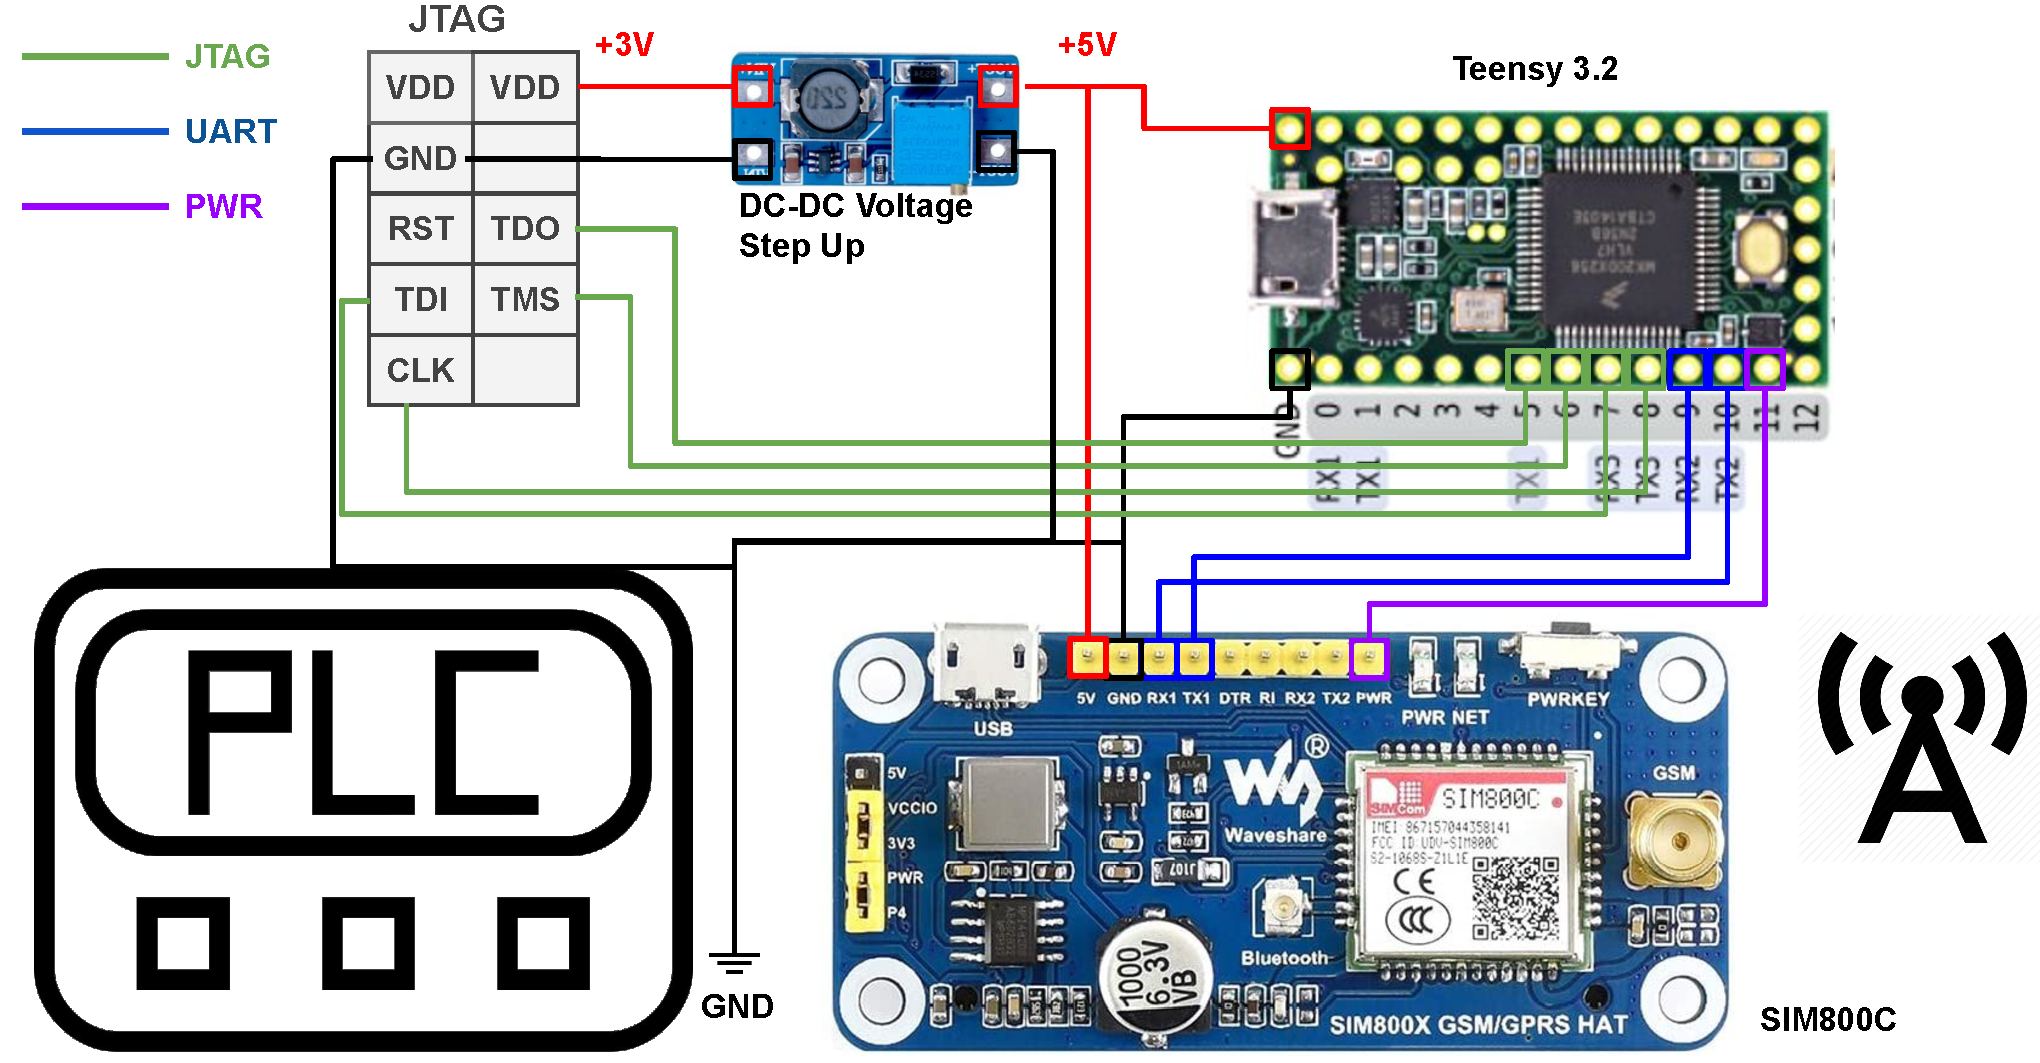
\includegraphics[width=0.47\textwidth]{figures/sim800teensy}
	\centering
	\caption{The power can be drawn from the JTAG pad or directly from the border connector p607. Since the JTAG pad provides the 3 volts source, we also need a DC-DC voltage step-up module that boosts from 3 volts to 5 volts. One GPIO pin from Teensy connects the PWR pin of the SIM800C board. It is used to deliver the power and reset sequence. After SIM800C initialized, the Teensy module sends AT commands through the serial port.}
	\label{fig:sim800teensy}
\end{figure}

The SIM800C is a Quad-Band GSM/GPRS module. It has strong extension capability with interfaces including UART, USB2.0, and GPIO. ~\autoref{fig:sim800teensy} shows that the SIM800C module connects with the Teensy board through a serial port. First, the Teensy boart initializes the cellular module using AT command, connecting to the network. Once a text message is received, the Teensy board reads it and looks for control commands. In such a case,  the command will be parsed as IO operations that eventually turn into particular memory read/write on PLC's GPIO port.

%! TEX root = 'main.tex'
\section{Implementation and Experiment}
\label{sec:implant-implementation}


This section provides the implementation details and discusses the issues that we encountered during the development. 
%We also give some experiments to prepare for attacks in different scenarios, which are not used in the current prototype.


\textbf{\texttt{Read/Write Memory.}} We briefly introduced the JTAG protocol in the background (~\autoref{sec:implant-background}) earlier. Our driver sends instructions to the IR and reads the returned result according to the JTAG state machine. Nevertheless, we need to know how to operate ARM's CoreSight components for this particular hardware backdoor prototype. We choose the JTAG interface instead of SW (Serial Wire), so the corresponding debug port is JTAG-DP or SWJ-DP, as shown in~\autoref{fig:dap}.

\begin{center}
	\begin{table}
		\small
		%\begin{tabular}{p{1.6cm}  p{1.6cm}  p{4cm}} 
		\begin{tabular}{l l l l} 
			\hline
			\makecell{IR \\ value} & \makecell{JTAG-DP \\ Register} & \makecell{DR \\ width} & Description  \\ 
			\hline
			%\multicolumn{3}{l}{\textbf{Memory} (0x00000000 - 0x22200000)}  \\
			%\hline
			b1000 & ABORT & 35 & JTAG-DP Abort Register \\
			\hline
			b1010 & DPACC & 35 & JTAG DP Access Register \\
			\hline
			b1011 & APACC & 35 & JTAG AP Access Register\\
			\hline
			b1110 & IDCODE & 32 & JTAG Device ID Code Register \\
			\hline
			b1111 & BYPASS & 1  & JTAG Bypass Register \\
			\hline
		\end{tabular}
		\caption{DPACC is used for Debug Port (DP) accesses. APACC is used for Access Port (AP) accesses, and it can access a register of a debug component of the system to which the interface is connected.}
		\label{tab:jtag-dp}
	\end{table}
\end{center}



Through DPACC and APACC registers, the debugger can access resources provided by other access ports (AP).  As mentioned earlier, an access port provides the interface between the debug port interface and one or more debug components present within the system. There are two kinds of access ports: Memory Access Ports (MEM-AP) and JTAG Access Ports (JTAG-AP), and MEM-AP is designed for connects to memory bus system with address and data controls.  Since our backdoor wants to access memory and GPIO, we need to access either AHB-AP or the MEM-AP, which handled the differences between the underlying bus.



\begin{figure}[ht]
	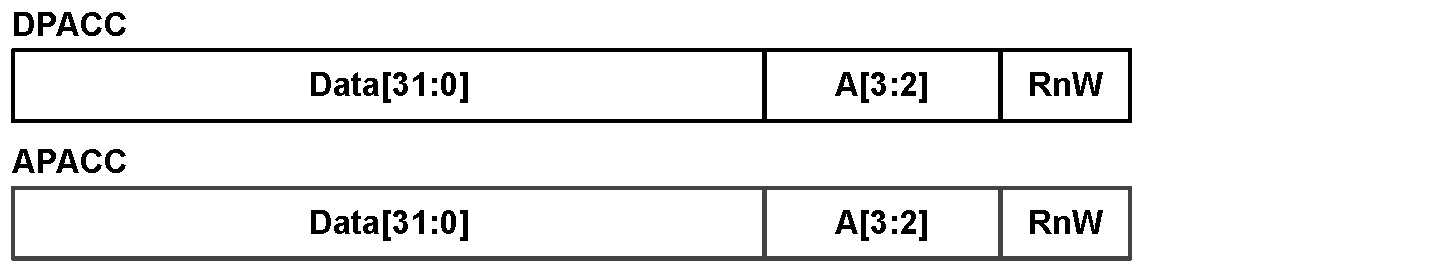
\includegraphics[width=0.47\textwidth]{figures/dpapacc}
	\centering
	\caption{Both of the two registers are 35 bits long and can be scanned in/out through the JTAG protocol with IR instruction b1010 and b1010, respectively. RnW takes one bit, and zero indicates a write. A[3:2] selects the register within a bank.}
	\label{fig:dpapacc}
\end{figure}


~\autoref{fig:dpapacc} shows that both DPACC and APACC have the same structure, and they can be scan in/out through the JTAG state machine with the specific IR instruction value. The lowest bit indicates whether to read or write DP/AP, where zero means write.

 According to ARM Debug Interface Architecture Specification v5.0 to v5.2, every bank has four registers, and A[3:2], the two bits are used to select the register from the bank. The DP only has one bank, and the MEM-AP has 16 banks, as listed in~\autoref{tab:dpreg} and ~\autoref{tab:memapreg}, respectively. To select the AP's bank, we also need to write the bank address into the DP's SELECT register.




\begin{center}
	\begin{table}
		\small
		%\begin{tabular}{p{1.6cm}  p{1.6cm}  p{4cm}} 
		\begin{tabular}{l l l} 
			\hline
			Offset & Register &  Description  \\ 
			\hline
			%\multicolumn{3}{l}{\textbf{Memory} (0x00000000 - 0x22200000)}  \\
			%\hline
			0x00 & & Reserved \\
			\hline
			0x04 & CTRL/STAT & Control and State Register \\
			\hline
			0x08 & SELECT & AP Select \\
			\hline
			0x0C & RDBUFF & Read Buffer\\
			\hline
		\end{tabular}
		\caption{Debug Port registers. Debug Port only has one bank, a total of four registers, which can be specified by A[3:2] of the DPACC register. }
		\label{tab:dpreg}
	\end{table}
\end{center}

\begin{center}
	\begin{table}
		\small
		%\begin{tabular}{p{1.6cm}  p{1.6cm}  p{4cm}} 
		\begin{tabular}{l l l} 
			\hline
			Offset & Register &  Description  \\ 
			\hline
			%\multicolumn{3}{l}{\textbf{Memory} (0x00000000 - 0x22200000)}  \\
			%\hline
			0x00 & CSW & Control/Status Word register \\
			\hline
			0x04 & TAR & Transfer Address Register \\
			\hline
			0x08 & & Reserved \\
			\hline
			0x0C & DRW & Data Read/Write register\\
			\hline
			... & & \\
			\hline
			0xFC & IDR & Data Identification register\\
			\hline
		\end{tabular}
		\caption{Part of Memory Access Port (MEM-AP) registers. MEM-AP has 16 banks, and each bank has four registers, which can be specified by A[3:2] of the APACC register. The bank needs to be specified by the DP:SELECT register.}
		\label{tab:memapreg}
	\end{table}
\end{center}





To read and write memory, we need to use the internal registers provided by the MEM-AP. Specifically, we need to sue CSW, TAR, DRW, and others. Since these registers are in the MEM-AP's bank 0, we must first use DPACC to select it. Take writing memory as an example. Next, we need to write the destination address to TAR and then write the value to DRW. ~\autoref{fig:memapwrite} shows a pseudo-code for writing memory.


\begin{figure}[ht]
	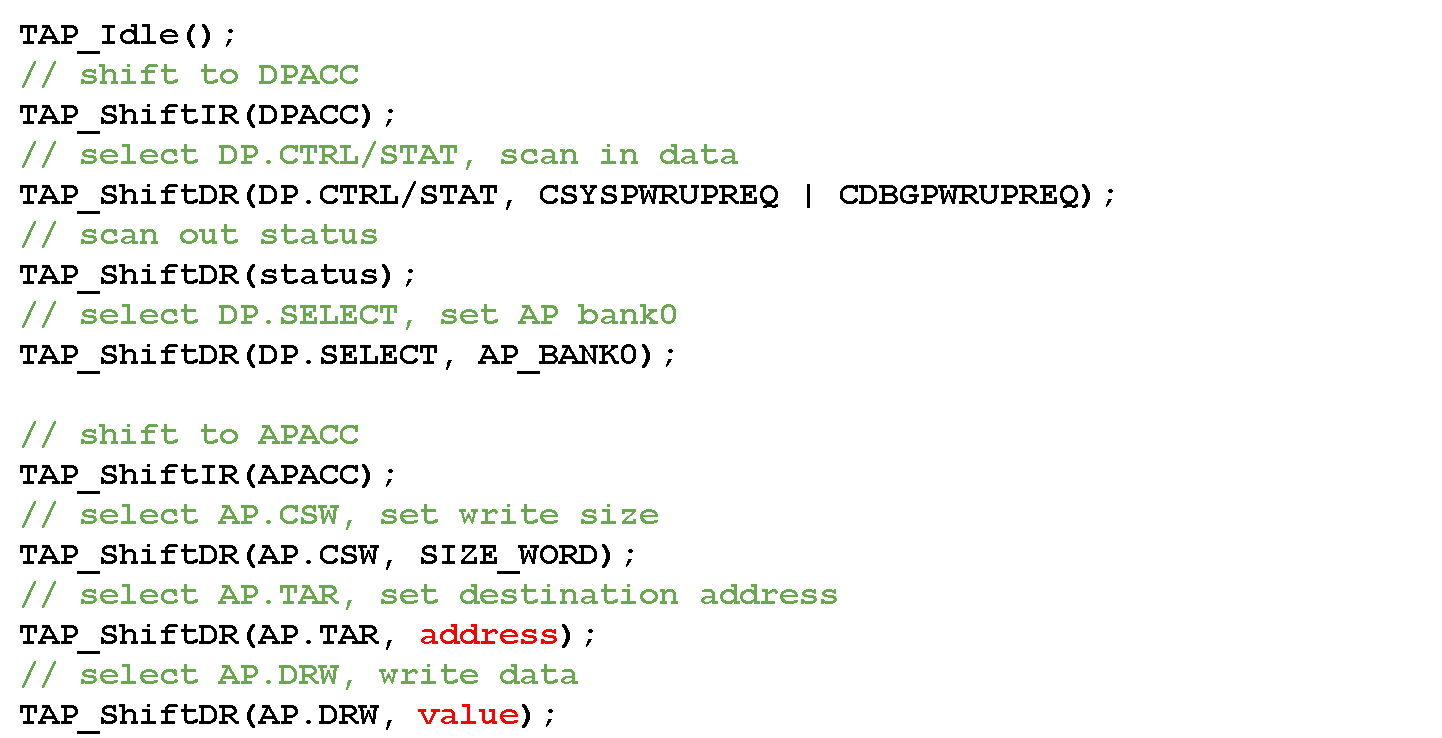
\includegraphics[width=0.47\textwidth]{figures/memapwrite2}
	\centering
	\caption{Pseudo-code for memory writing through MEM-AP. Notice, CSW, TAR and DRW are all in the bank zero. However, the bank is specified in the DP.SELECT instead of a register in AP.}
	\label{fig:memapwrite}
\end{figure}




\textbf{\texttt{Send/Receive SMS Message.}} SIM800C provides a serial port as the interface to receive AT commands. When \name is started, we use the AT+CMGF command to set the GSM chip in SMS Text Mode. Then we use the AT+CNMI command to set how to notify when new messages come. After that, the Teensy board keeps checking the serial port for new messages every second. If there is one, read the content and parse if it is a pre-defined attack command.

To send out a message, use the AT+CMGS command to set the destination phone number and then send the text message to the serial port. 


\textbf{\texttt{Intercepting SPI Data.}} As mentioned earlier, we can directly control the power switch chips to change the output or modify the transmission data by intercepting the bus on the circuit board, mainly low-speed buses such as SPI. For example, if we change a pin from zero to one, we need to connect it to the high voltage (3.3v) power supply to override the original signal. Similarly, we ground it to force it a zero. 
However, these operations need to consider the IC's interface.

The pins of the SPI flash chip use a push-pull configuration rather than an open drain. The output pins can actively create their own logical high and low states instead of relying on pull-up resistors to generate a default state. However, in this way, we must add an appropriate current-limiting resistor when forcing the signal to the ground or power supply to avoid short circuits.

For the SPI protocol, we modify the MOSI data line according to the SCLK clock signal, and we use FPGA to implement this circuit. In each clock cycle of SPI, we first read the data transmitted on the MOSI and store it into a shift register. When finding the target pattern, we modify the following data. To meet the setup time required for the SPI data line, we choose to make the circuits work on the clock's falling edge, given that the SPI works on the rising edge.

%! TEX root = 'main.tex'
\section{Evaluation}
\label{sec:evaluation}

\begin{figure}[th]
	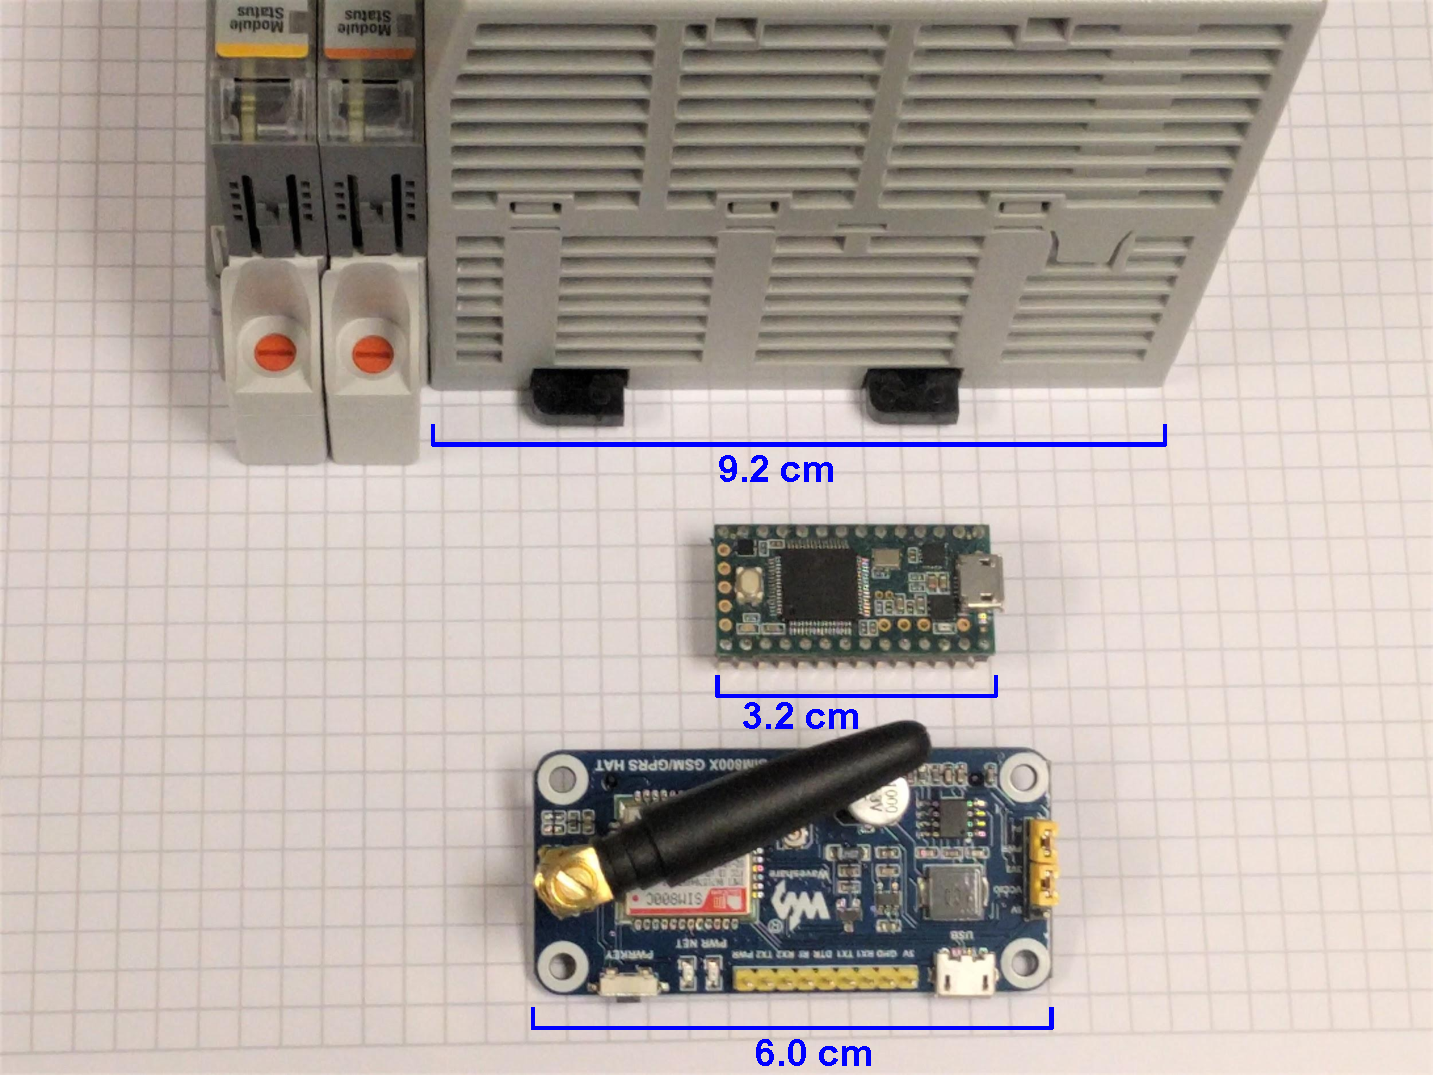
\includegraphics[width=0.47\textwidth]{figures/eval_size}
	\centering
	\caption{Test}
	\label{fig:eval_size}
\end{figure}


In our threat model, this hardware implant should exist independently of the PLC's communication network. To achieve this, as mentioned before, we chose to use cellular networks to communicate with nodes via SMS message. This approach is not as reliable as wired networks, especially in our attack model, which may require multiple nodes to launch attacks at the same time. We evaluated the approximate time required for SMS transmission, as shown in~\autoref{fig:smstime}, although we know that this may be affected by a variety of factors, such as the distance between the cell phone and the base station, the number of cell phones served by the same base station, across different networks, and so on. We also know that a SMS message over 160 characters will be split, large messages are segmented into 153 character segments and sent individually then rebuilt by the recipients device. But in order to avoid differences in the protocols implemented by different SMS programs or there may be some extra bytes attached to the SMS message, we did not strictly evaluate it by the number of SMS segments. From a practical point of view, we evaluated the transmission time corresponding to the length of the control command.

\begin{figure}[th]
	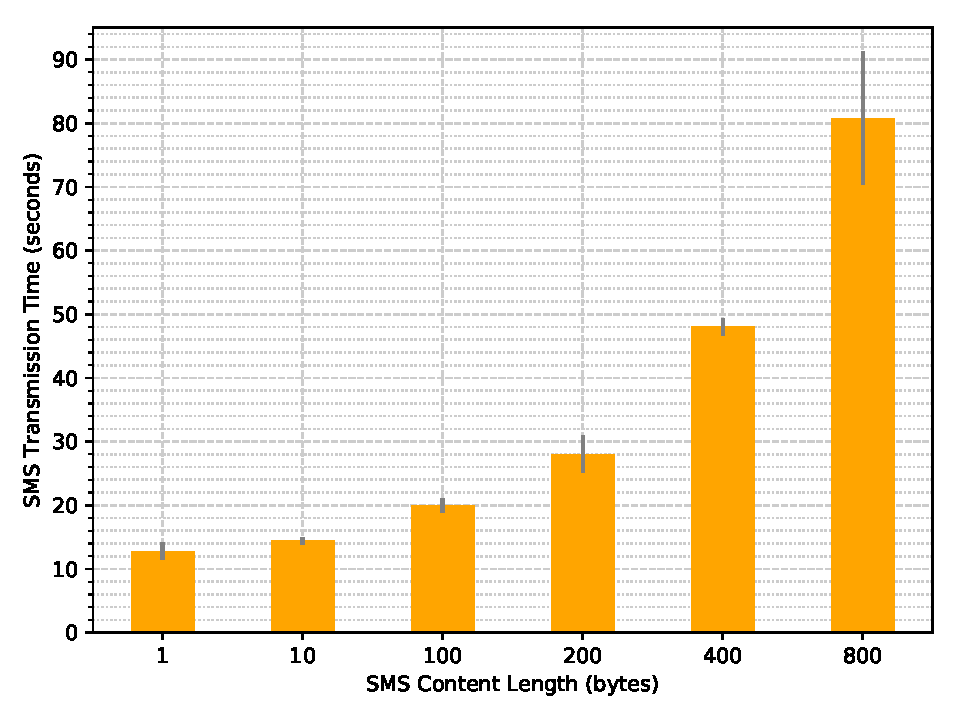
\includegraphics[width=0.47\textwidth]{figures/smstime}
	\centering
	\caption{SMS Message Transmission Time}
	\label{fig:smstime}
\end{figure}

The control command length can be only one byte, which is used to start a malicious function preset in the hardware implant. It can also be very long, such as containing a piece of binary to update the firmware of the PLC. Or it can contain a series of detailed attack instructions. The advantage of this is that even if the hardware implant is exposed, it does not contain specific attack instructions, thus avoiding further exposure to subsequence attacks and methods.

We get the data by sending a control command to a node with a phone. The command for each length was tested 20 times to obtain the mean and standard deviation. The cellular networks we used is T-Mobile and Google Fi. 

As shown in the figure, the longer the length of the control command, the more time it takes, and the less reliable it is for an attack that requires precise synchronization.


The hardware implant is powered directly from the PLC and does not consume a lot of power. The power consumption will only increase slightly when starting and executing the attack command, as shown in~\autoref{fig:current}.

\begin{figure*}[tp]
	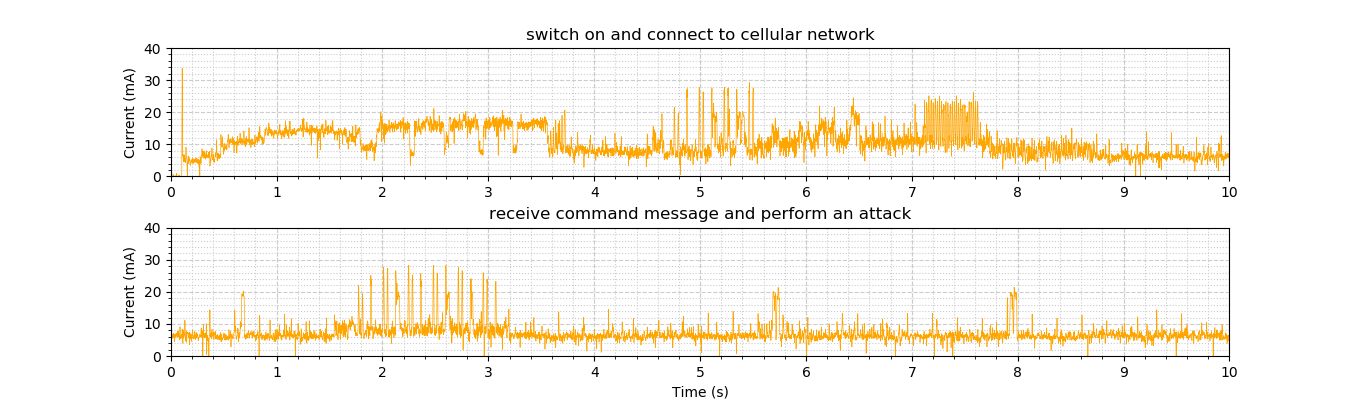
\includegraphics[width=\textwidth]{figures/current}
	\centering
	\caption{The hardware implant does not consume a lot of power, and the power consumption will only increase slightly when starting and executing the attack command.  }
	\label{fig:current}
\end{figure*}

%! TEX root = 'main.tex'
\section{Discussions and Mitigations}
\label{sec:implant-discussion}

Reducing the size of the hardware implant is necessary but not the main factor in disguising. A customized PCB board allows all the required chips to be installed together so that there is no Dupont jumper wire, which makes the hardware implant very suspicious. The SIM800C chip already is a SiP (System in a Package), and the JTAG driver can run on a minimal core such as cortex-M0. Combining these two can make the backdoor simpler, and we can already find such WIFI chips, such as ESP32~\cite{pravalika2019internet}, as of the time of writing this paper. Moreover, a better camouflage makes the hardware backdoor look like a legit accessory of the PLC. The IPMI (Intelligent Platform Management Interface) module is a good example. It needs to be purchased separately and installed on the reserved socket on the server motherboard to activate the remote control function.

To mitigate a hardware backdoor attack such as \name, we first measure the power usage to find the overhead caused by the extra circuitry, as evaluated in ~\autoref{implant-evaluation}. The result shows a few current peaks when \name connects to the GSM network and sends JTAG commands to PLC. However, its power consumed is not much, a few milliamperes. Moreover, the PLC's power consumption is also constantly fluctuating, and setting a threshold with little redundancy will affect the system's reliability.

In particular, to avoid malicious use of the JTAG interface, the manufacturer can blow the corresponding physical JTAG fuse at the factory~\cite{rosenfeld2010attacks}~\cite{buskey2006protected}. Blowing the fuse completely disables the JTAG port and is not reversible.

However, by tapping the open wire on the boards, we can directly control each peripheral device because they are connected to the microcontroller through various buses. We think that some physical protection will cause trouble to the attacker. For example, the Chip-on-Board (COB)~\cite{lau1994chip} packaging with a black blob for low-cost IC items makes it more challenging to identify the chip underneath. Nevertheless, we believe it is not a good practice to cover the whole board, and heat dissipation is critical for large area ICs. One possible direction for preventing bus signal hijacking is to send packet-based encrypted data, which requires the microcontroller and peripherals to exchange encryption keys and maintain a connection state. However, it may not be practical for low-speed devices and low-end microcontrollers.


%! TEX root = 'main.tex'
\section{Related Work}
\label{sec:implant-relatedwork}



Firmware modification attacks~\cite{newman2011scada, basnight2013firmware, blanco2012one, cui2013firmware, konstantinou2015impact, schulz2017nexmon} constitute significant attacks targeting embedded systems, industrial control systems, and IoT devices. 

Harvey~\cite{garcia2017hey} is a physical-aware stealthy rootkit against a cyber-physical power grid control system. It hides within the PLC's firmware below the control logic and modifies control commands before sending it to the physical plant's actuators. This work~\cite{moore2017implications} implements a malicious firmware that ignored incoming print commands for a printed 3D model, substitutes malicious print commands for an alternate 3D model.  If the firmware attacks can be carried out remotely, the harm will be even more significant. Cui et al.~\cite{cui2013firmware} gives a detailed case study of the HP-RFU (Remote Firmware Update) LaserJet printer firmware modification vulnerability, which allows arbitrary injection of malware into the printer's firmware via standard printed documents.

These systems have one thing in common: they all run on a microcontroller with limited computing power. Therefore, these devices run a simple real-time operating system, and there has not been a complete anti-virus system or a series of integrity verification features and programs provided by hardware and operating system like those on modern PCs. Due to the lack of security features, the programs run on those systems are often more vulnerable. Moreover, because they usually focus on specific areas and are not easily accessible, security issues are ignored. However, once those systems are compromised, through firmware modification, the attacker can stay in the dark for a long time without being discovered and cause a significant impact at a particular moment.

On the other hand, there are many ways to protect the firmware from being modified. ConFirm~\cite{wang2015confirm} is a low-cost technique to detect malicious modifications in the firmware of embedded control systems. It measures the number of low-level hardware events that occur during the execution of the firmware. Lee et al.~\cite{lee2016binding} presented a technique for binding software to hardware instances that use the devices' hardware security properties. The proposed technique assures manufacturers that only they can perform their hardware and software binding and create their products.

Remote software attestation~\cite{li2011viper} is also a defense against firmware modification.  SWATT~\cite{seshadri2004swatt} verifies embedded devices' memory contents and establishes the absence of malicious changes to the memory contents without using extra security hardware features. It uses a challenge-response protocol between the
verifier and the embedded device. The verifier sends a challenge to the embedded device. The embedded device computes a response to this challenge in a pre-defined protocol between the verifier and the device. The device can only give the correct answer if the memory content is intact. Otherwise, the attacker has to know the verifier's secret algorithm to break the verification. Similarly, SBAP~\cite{li2010sbap} also provides a software-only solution to verify the firmware integrity but with the help of an existing peripheral device.

Other methods, such as firmware binary obfuscation~\cite{cyr2019low, schrittwieser2016protecting, cheng2019dynopvm}, make it very challenging for firmware modification attacks. It requires comprehensively analyzing each device to find a suitable place to inject malicious code.

%%\input{sources/limitationfuturework}

%! TEX root = 'main.tex'
\section{Conclusions}
\label{sec:implant-conclusions}

To achieve more stealthiness in a sophisticated APT attack, we think the trend is that the trojan moves towards the hardware level, especially with the emerging supply chain attacks. We present \name, a parasitical hardware implant that directly controls the PLC through wire and bus signal hijacking. \name does not modify the firmware nor relies on PLC's network communication. It can manage/damage the ICS system's physical assets by controlling PLC's IO.  At the same time, it provides a faked expected view of the system to circumvent detections. Our prototype is small in size, and the experiment results demonstrate the feasibility of \name in practice.


% uty


%\section{Introduction}
%ACM's consolidated article template, introduced in 2017, provides a
%consistent \LaTeX\ style for use across ACM publications, and
%incorporates accessibility and metadata-extraction functionality
%necessary for future Digital Library endeavors. Numerous ACM and
%SIG-specific \LaTeX\ templates have been examined, and their unique
%features incorporated into this single new template.
%
%If you are new to publishing with ACM, this document is a valuable
%guide to the process of preparing your work for publication. If you
%have published with ACM before, this document provides insight and
%instruction into more recent changes to the article template.
%
%The ``\verb|acmart|'' document class can be used to prepare articles
%for any ACM publication --- conference or journal, and for any stage
%of publication, from review to final ``camera-ready'' copy, to the
%author's own version, with {\itshape very} few changes to the source.
%
%\section{Template Overview}
%As noted in the introduction, the ``\verb|acmart|'' document class can
%be used to prepare many different kinds of documentation --- a
%double-blind initial submission of a full-length technical paper, a
%two-page SIGGRAPH Emerging Technologies abstract, a ``camera-ready''
%journal article, a SIGCHI Extended Abstract, and more --- all by
%selecting the appropriate {\itshape template style} and {\itshape
%  template parameters}.
%
%This document will explain the major features of the document
%class. For further information, the {\itshape \LaTeX\ User's Guide} is
%available from
%\url{https://www.acm.org/publications/proceedings-template}.
%
%\subsection{Template Styles}
%
%The primary parameter given to the ``\verb|acmart|'' document class is
%the {\itshape template style} which corresponds to the kind of publication
%or SIG publishing the work. This parameter is enclosed in square
%brackets and is a part of the {\verb|documentclass|} command:
%\begin{verbatim}
%  \documentclass[STYLE]{acmart}
%\end{verbatim}
%
%Journals use one of three template styles. All but three ACM journals
%use the {\verb|acmsmall|} template style:
%\begin{itemize}
%\item {\verb|acmsmall|}: The default journal template style.
%\item {\verb|acmlarge|}: Used by JOCCH and TAP.
%\item {\verb|acmtog|}: Used by TOG.
%\end{itemize}
%
%The majority of conference proceedings documentation will use the {\verb|acmconf|} template style.
%\begin{itemize}
%\item {\verb|acmconf|}: The default proceedings template style.
%\item{\verb|sigchi|}: Used for SIGCHI conference articles.
%\item{\verb|sigchi-a|}: Used for SIGCHI ``Extended Abstract'' articles.
%\item{\verb|sigplan|}: Used for SIGPLAN conference articles.
%\end{itemize}
%
%\subsection{Template Parameters}
%
%In addition to specifying the {\itshape template style} to be used in
%formatting your work, there are a number of {\itshape template parameters}
%which modify some part of the applied template style. A complete list
%of these parameters can be found in the {\itshape \LaTeX\ User's Guide.}
%
%Frequently-used parameters, or combinations of parameters, include:
%\begin{itemize}
%\item {\verb|anonymous,review|}: Suitable for a ``double-blind''
%  conference submission. Anonymizes the work and includes line
%  numbers. Use with the \verb|\acmSubmissionID| command to print the
%  submission's unique ID on each page of the work.
%\item{\verb|authorversion|}: Produces a version of the work suitable
%  for posting by the author.
%\item{\verb|screen|}: Produces colored hyperlinks.
%\end{itemize}
%
%This document uses the following string as the first command in the
%source file:
%\begin{verbatim}
%\documentclass[sigconf]{acmart}
%\end{verbatim}
%
%\section{Modifications}
%
%Modifying the template --- including but not limited to: adjusting
%margins, typeface sizes, line spacing, paragraph and list definitions,
%and the use of the \verb|\vspace| command to manually adjust the
%vertical spacing between elements of your work --- is not allowed.
%
%{\bfseries Your document will be returned to you for revision if
%  modifications are discovered.}
%
%\section{Typefaces}
%
%The ``\verb|acmart|'' document class requires the use of the
%``Libertine'' typeface family. Your \TeX\ installation should include
%this set of packages. Please do not substitute other typefaces. The
%``\verb|lmodern|'' and ``\verb|ltimes|'' packages should not be used,
%as they will override the built-in typeface families.
%
%\section{Title Information}
%
%The title of your work should use capital letters appropriately -
%\url{https://capitalizemytitle.com/} has useful rules for
%capitalization. Use the {\verb|title|} command to define the title of
%your work. If your work has a subtitle, define it with the
%{\verb|subtitle|} command.  Do not insert line breaks in your title.
%
%If your title is lengthy, you must define a short version to be used
%in the page headers, to prevent overlapping text. The \verb|title|
%command has a ``short title'' parameter:
%\begin{verbatim}
%  \title[short title]{full title}
%\end{verbatim}
%
%\section{Authors and Affiliations}
%
%Each author must be defined separately for accurate metadata
%identification. Multiple authors may share one affiliation. Authors'
%names should not be abbreviated; use full first names wherever
%possible. Include authors' e-mail addresses whenever possible.
%
%Grouping authors' names or e-mail addresses, or providing an ``e-mail
%alias,'' as shown below, is not acceptable:
%\begin{verbatim}
%  \author{Brooke Aster, David Mehldau}
%  \email{dave,judy,steve@university.edu}
%  \email{firstname.lastname@phillips.org}
%\end{verbatim}
%
%The \verb|authornote| and \verb|authornotemark| commands allow a note
%to apply to multiple authors --- for example, if the first two authors
%of an article contributed equally to the work.
%
%If your author list is lengthy, you must define a shortened version of
%the list of authors to be used in the page headers, to prevent
%overlapping text. The following command should be placed just after
%the last \verb|\author{}| definition:
%\begin{verbatim}
%  \renewcommand{\shortauthors}{McCartney, et al.}
%\end{verbatim}
%Omitting this command will force the use of a concatenated list of all
%of the authors' names, which may result in overlapping text in the
%page headers.
%
%The article template's documentation, available at
%\url{https://www.acm.org/publications/proceedings-template}, has a
%complete explanation of these commands and tips for their effective
%use.
%
%Note that authors' addresses are mandatory for journal articles.
%
%\section{Rights Information}
%
%Authors of any work published by ACM will need to complete a rights
%form. Depending on the kind of work, and the rights management choice
%made by the author, this may be copyright transfer, permission,
%license, or an OA (open access) agreement.
%
%Regardless of the rights management choice, the author will receive a
%copy of the completed rights form once it has been submitted. This
%form contains \LaTeX\ commands that must be copied into the source
%document. When the document source is compiled, these commands and
%their parameters add formatted text to several areas of the final
%document:
%\begin{itemize}
%\item the ``ACM Reference Format'' text on the first page.
%\item the ``rights management'' text on the first page.
%\item the conference information in the page header(s).
%\end{itemize}
%
%Rights information is unique to the work; if you are preparing several
%works for an event, make sure to use the correct set of commands with
%each of the works.
%
%The ACM Reference Format text is required for all articles over one
%page in length, and is optional for one-page articles (abstracts).
%
%\section{CCS Concepts and User-Defined Keywords}
%
%Two elements of the ``acmart'' document class provide powerful
%taxonomic tools for you to help readers find your work in an online
%search.
%
%The ACM Computing Classification System ---
%\url{https://www.acm.org/publications/class-2012} --- is a set of
%classifiers and concepts that describe the computing
%discipline. Authors can select entries from this classification
%system, via \url{https://dl.acm.org/ccs/ccs.cfm}, and generate the
%commands to be included in the \LaTeX\ source.
%
%User-defined keywords are a comma-separated list of words and phrases
%of the authors' choosing, providing a more flexible way of describing
%the research being presented.
%
%CCS concepts and user-defined keywords are required for for all
%articles over two pages in length, and are optional for one- and
%two-page articles (or abstracts).
%
%\section{Sectioning Commands}
%
%Your work should use standard \LaTeX\ sectioning commands:
%\verb|section|, \verb|subsection|, \verb|subsubsection|, and
%\verb|paragraph|. They should be numbered; do not remove the numbering
%from the commands.
%
%Simulating a sectioning command by setting the first word or words of
%a paragraph in boldface or italicized text is {\bfseries not allowed.}
%
%\section{Tables}
%
%The ``\verb|acmart|'' document class includes the ``\verb|booktabs|''
%package --- \url{https://ctan.org/pkg/booktabs} --- for preparing
%high-quality tables.
%
%Table captions are placed {\itshape above} the table.
%
%Because tables cannot be split across pages, the best placement for
%them is typically the top of the page nearest their initial cite.  To
%ensure this proper ``floating'' placement of tables, use the
%environment \textbf{table} to enclose the table's contents and the
%table caption.  The contents of the table itself must go in the
%\textbf{tabular} environment, to be aligned properly in rows and
%columns, with the desired horizontal and vertical rules.  Again,
%detailed instructions on \textbf{tabular} material are found in the
%\textit{\LaTeX\ User's Guide}.
%
%Immediately following this sentence is the point at which
%Table~\ref{tab:freq} is included in the input file; compare the
%placement of the table here with the table in the printed output of
%this document.
%
%\begin{table}
%  \caption{Frequency of Special Characters}
%  \label{tab:freq}
%  \begin{tabular}{ccl}
%    \toprule
%    Non-English or Math&Frequency&Comments\\
%    \midrule
%    \O & 1 in 1,000& For Swedish names\\
%    $\pi$ & 1 in 5& Common in math\\
%    \$ & 4 in 5 & Used in business\\
%    $\Psi^2_1$ & 1 in 40,000& Unexplained usage\\
%  \bottomrule
%\end{tabular}
%\end{table}
%
%To set a wider table, which takes up the whole width of the page's
%live area, use the environment \textbf{table*} to enclose the table's
%contents and the table caption.  As with a single-column table, this
%wide table will ``float'' to a location deemed more
%desirable. Immediately following this sentence is the point at which
%Table~\ref{tab:commands} is included in the input file; again, it is
%instructive to compare the placement of the table here with the table
%in the printed output of this document.
%
%\begin{table*}
%  \caption{Some Typical Commands}
%  \label{tab:commands}
%  \begin{tabular}{ccl}
%    \toprule
%    Command &A Number & Comments\\
%    \midrule
%    \texttt{{\char'134}author} & 100& Author \\
%    \texttt{{\char'134}table}& 300 & For tables\\
%    \texttt{{\char'134}table*}& 400& For wider tables\\
%    \bottomrule
%  \end{tabular}
%\end{table*}
%
%Always use midrule to separate table header rows from data rows, and
%use it only for this purpose. This enables assistive technologies to
%recognise table headers and support their users in navigating tables
%more easily.
%
%\section{Math Equations}
%You may want to display math equations in three distinct styles:
%inline, numbered or non-numbered display.  Each of the three are
%discussed in the next sections.
%
%\subsection{Inline (In-text) Equations}
%A formula that appears in the running text is called an inline or
%in-text formula.  It is produced by the \textbf{math} environment,
%which can be invoked with the usual
%\texttt{{\char'134}begin\,\ldots{\char'134}end} construction or with
%the short form \texttt{\$\,\ldots\$}. You can use any of the symbols
%and structures, from $\alpha$ to $\omega$, available in
%\LaTeX~\cite{Lamport:LaTeX}; this section will simply show a few
%examples of in-text equations in context. Notice how this equation:
%\begin{math}
%  \lim_{n\rightarrow \infty}x=0
%\end{math},
%set here in in-line math style, looks slightly different when
%set in display style.  (See next section).
%
%\subsection{Display Equations}
%A numbered display equation---one set off by vertical space from the
%text and centered horizontally---is produced by the \textbf{equation}
%environment. An unnumbered display equation is produced by the
%\textbf{displaymath} environment.
%
%Again, in either environment, you can use any of the symbols and
%structures available in \LaTeX\@; this section will just give a couple
%of examples of display equations in context.  First, consider the
%equation, shown as an inline equation above:
%\begin{equation}
%  \lim_{n\rightarrow \infty}x=0
%\end{equation}
%Notice how it is formatted somewhat differently in
%the \textbf{displaymath}
%environment.  Now, we'll enter an unnumbered equation:
%\begin{displaymath}
%  \sum_{i=0}^{\infty} x + 1
%\end{displaymath}
%and follow it with another numbered equation:
%\begin{equation}
%  \sum_{i=0}^{\infty}x_i=\int_{0}^{\pi+2} f
%\end{equation}
%just to demonstrate \LaTeX's able handling of numbering.
%
%\section{Figures}
%
%The ``\verb|figure|'' environment should be used for figures. One or
%more images can be placed within a figure. If your figure contains
%third-party material, you must clearly identify it as such, as shown
%in the example below.
%\begin{figure}[h]
%  \centering
%  \includegraphics[width=\linewidth]{sample-franklin}
%  \caption{1907 Franklin Model D roadster. Photograph by Harris \&
%    Ewing, Inc. [Public domain], via Wikimedia
%    Commons. (\url{https://goo.gl/VLCRBB}).}
%  \Description{A woman and a girl in white dresses sit in an open car.}
%\end{figure}
%
%Your figures should contain a caption which describes the figure to
%the reader.
%
%Figure captions are placed {\itshape below} the figure.
%
%Every figure should also have a figure description unless it is purely
%decorative. These descriptions convey what’s in the image to someone
%who cannot see it. They are also used by search engine crawlers for
%indexing images, and when images cannot be loaded.
%
%A figure description must be unformatted plain text less than 2000
%characters long (including spaces).  {\bfseries Figure descriptions
%  should not repeat the figure caption – their purpose is to capture
%  important information that is not already provided in the caption or
%  the main text of the paper.} For figures that convey important and
%complex new information, a short text description may not be
%adequate. More complex alternative descriptions can be placed in an
%appendix and referenced in a short figure description. For example,
%provide a data table capturing the information in a bar chart, or a
%structured list representing a graph.  For additional information
%regarding how best to write figure descriptions and why doing this is
%so important, please see
%\url{https://www.acm.org/publications/taps/describing-figures/}.
%
%\subsection{The ``Teaser Figure''}
%
%A ``teaser figure'' is an image, or set of images in one figure, that
%are placed after all author and affiliation information, and before
%the body of the article, spanning the page. If you wish to have such a
%figure in your article, place the command immediately before the
%\verb|\maketitle| command:
%\begin{verbatim}
%  \begin{teaserfigure}
%    \includegraphics[width=\textwidth]{sampleteaser}
%    \caption{figure caption}
%    \Description{figure description}
%  \end{teaserfigure}
%\end{verbatim}
%
%\section{Citations and Bibliographies}
%
%The use of \BibTeX\ for the preparation and formatting of one's
%references is strongly recommended. Authors' names should be complete
%--- use full first names (``Donald E. Knuth'') not initials
%(``D. E. Knuth'') --- and the salient identifying features of a
%reference should be included: title, year, volume, number, pages,
%article DOI, etc.
%
%The bibliography is included in your source document with these two
%commands, placed just before the \verb|\end{document}| command:
%\begin{verbatim}
%  \bibliographystyle{ACM-Reference-Format}
%  \bibliography{bibfile}
%\end{verbatim}
%where ``\verb|bibfile|'' is the name, without the ``\verb|.bib|''
%suffix, of the \BibTeX\ file.
%
%Citations and references are numbered by default. A small number of
%ACM publications have citations and references formatted in the
%``author year'' style; for these exceptions, please include this
%command in the {\bfseries preamble} (before the command
%``\verb|\begin{document}|'') of your \LaTeX\ source:
%\begin{verbatim}
%  \citestyle{acmauthoryear}
%\end{verbatim}
%
%  Some examples.  A paginated journal article \cite{Abril07}, an
%  enumerated journal article \cite{Cohen07}, a reference to an entire
%  issue \cite{JCohen96}, a monograph (whole book) \cite{Kosiur01}, a
%  monograph/whole book in a series (see 2a in spec. document)
%  \cite{Harel79}, a divisible-book such as an anthology or compilation
%  \cite{Editor00} followed by the same example, however we only output
%  the series if the volume number is given \cite{Editor00a} (so
%  Editor00a's series should NOT be present since it has no vol. no.),
%  a chapter in a divisible book \cite{Spector90}, a chapter in a
%  divisible book in a series \cite{Douglass98}, a multi-volume work as
%  book \cite{Knuth97}, a couple of articles in a proceedings (of a
%  conference, symposium, workshop for example) (paginated proceedings
%  article) \cite{Andler79, Hagerup1993}, a proceedings article with
%  all possible elements \cite{Smith10}, an example of an enumerated
%  proceedings article \cite{VanGundy07}, an informally published work
%  \cite{Harel78}, a couple of preprints \cite{Bornmann2019,
%    AnzarootPBM14}, a doctoral dissertation \cite{Clarkson85}, a
%  master's thesis: \cite{anisi03}, an online document / world wide web
%  resource \cite{Thornburg01, Ablamowicz07, Poker06}, a video game
%  (Case 1) \cite{Obama08} and (Case 2) \cite{Novak03} and \cite{Lee05}
%  and (Case 3) a patent \cite{JoeScientist001}, work accepted for
%  publication \cite{rous08}, 'YYYYb'-test for prolific author
%  \cite{SaeediMEJ10} and \cite{SaeediJETC10}. Other cites might
%  contain 'duplicate' DOI and URLs (some SIAM articles)
%  \cite{Kirschmer:2010:AEI:1958016.1958018}. Boris / Barbara Beeton:
%  multi-volume works as books \cite{MR781536} and \cite{MR781537}. A
%  couple of citations with DOIs:
%  \cite{2004:ITE:1009386.1010128,Kirschmer:2010:AEI:1958016.1958018}. Online
%  citations: \cite{TUGInstmem, Thornburg01, CTANacmart}. Artifacts:
%  \cite{R} and \cite{UMassCitations}.
%
%\section{Acknowledgments}
%
%Identification of funding sources and other support, and thanks to
%individuals and groups that assisted in the research and the
%preparation of the work should be included in an acknowledgment
%section, which is placed just before the reference section in your
%document.
%
%This section has a special environment:
%\begin{verbatim}
%  \begin{acks}
%  ...
%  \end{acks}
%\end{verbatim}
%so that the information contained therein can be more easily collected
%during the article metadata extraction phase, and to ensure
%consistency in the spelling of the section heading.
%
%Authors should not prepare this section as a numbered or unnumbered {\verb|\section|}; please use the ``{\verb|acks|}'' environment.
%
%\section{Appendices}
%
%If your work needs an appendix, add it before the
%``\verb|\end{document}|'' command at the conclusion of your source
%document.
%
%Start the appendix with the ``\verb|appendix|'' command:
%\begin{verbatim}
%  \appendix
%\end{verbatim}
%and note that in the appendix, sections are lettered, not
%numbered. This document has two appendices, demonstrating the section
%and subsection identification method.
%
%\section{SIGCHI Extended Abstracts}
%
%The ``\verb|sigchi-a|'' template style (available only in \LaTeX\ and
%not in Word) produces a landscape-orientation formatted article, with
%a wide left margin. Three environments are available for use with the
%``\verb|sigchi-a|'' template style, and produce formatted output in
%the margin:
%\begin{itemize}
%\item {\verb|sidebar|}:  Place formatted text in the margin.
%\item {\verb|marginfigure|}: Place a figure in the margin.
%\item {\verb|margintable|}: Place a table in the margin.
%\end{itemize}
%
%%%
%%% The acknowledgments section is defined using the "acks" environment
%%% (and NOT an unnumbered section). This ensures the proper
%%% identification of the section in the article metadata, and the
%%% consistent spelling of the heading.
%\begin{acks}
%To Robert, for the bagels and explaining CMYK and color spaces.
%\end{acks}

%%
%% The next two lines define the bibliography style to be used, and
%% the bibliography file.
\bibliographystyle{ACM-Reference-Format}
%\bibliography{sample-base}
\bibliography{bib.bib}


%\newpage
%%! TEX root = 'main.tex'
\appendix

\begin{appendices}

\section{}
\label{sec:implant-appendix}



\begin{figure*}[hb!]
	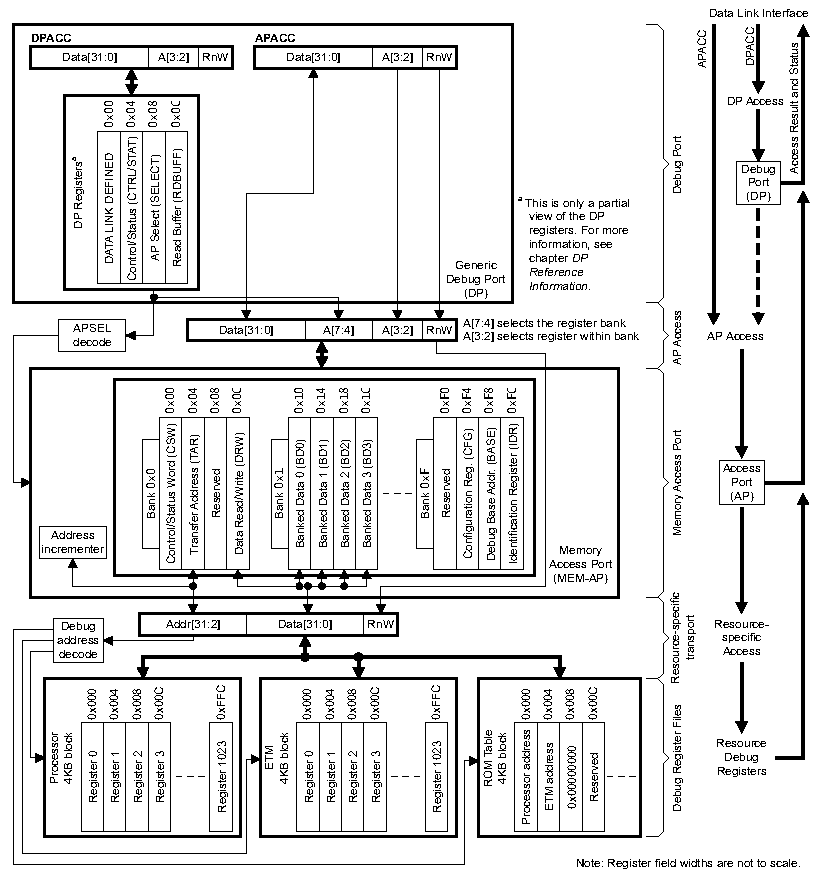
\includegraphics[width=0.9\textwidth]{figures/memap}
	\centering
	\caption{MEM-AP connecting the DP to debug components. This figure is available in the ARM Debug Interface Architecture Specification.}
	\label{fig:memap}
\end{figure*}


\end{appendices}

% uty

%%
%% If your work has an appendix, this is the place to put it.
%\appendix
%
%\section{Research Methods}
%
%\subsection{Part One}
%
%Lorem ipsum dolor sit amet, consectetur adipiscing elit. Morbi
%malesuada, quam in pulvinar varius, metus nunc fermentum urna, id
%sollicitudin purus odio sit amet enim. Aliquam ullamcorper eu ipsum
%vel mollis. Curabitur quis dictum nisl. Phasellus vel semper risus, et
%lacinia dolor. Integer ultricies commodo sem nec semper.
%
%\subsection{Part Two}
%
%Etiam commodo feugiat nisl pulvinar pellentesque. Etiam auctor sodales
%ligula, non varius nibh pulvinar semper. Suspendisse nec lectus non
%ipsum convallis congue hendrerit vitae sapien. Donec at laoreet
%eros. Vivamus non purus placerat, scelerisque diam eu, cursus
%ante. Etiam aliquam tortor auctor efficitur mattis.
%
%\section{Online Resources}
%
%Nam id fermentum dui. Suspendisse sagittis tortor a nulla mollis, in
%pulvinar ex pretium. Sed interdum orci quis metus euismod, et sagittis
%enim maximus. Vestibulum gravida massa ut felis suscipit
%congue. Quisque mattis elit a risus ultrices commodo venenatis eget
%dui. Etiam sagittis eleifend elementum.
%
%Nam interdum magna at lectus dignissim, ac dignissim lorem
%rhoncus. Maecenas eu arcu ac neque placerat aliquam. Nunc pulvinar
%massa et mattis lacinia.

\end{document}
\endinput
%%
%% End of file `sample-sigconf.tex'.
